\chapter{Integration of R-STDP and Federated Learning}

\section{Consensus Flying Problem}

This chapter studies the cooperation between follower drones to follow the leader drone by integrating \ac{stdp} and \ac{fl}. The cooperation problem is formation flying or ``Consensus Flying". The consensus flying problem deals with ensuring drones can work together in real-time to agree on their flight paths and positions. When many drones are close together, like in swarms, avoiding crashes is vital. Advanced algorithms and communication methods are needed so drones can exchange information and handle changing situations and unexpected obstacles.

As shown in Figure \ref{fig.Consensus Flying}, a swarm of agents (follower drones) flies around a leader. The leader is controlled from a remote base station, and the swarm agents should learn to fly safely with the leader. The leader sends its position to all agents, and each agent only sees two neighboring agents. The swarm aims to learn how to keep a commanded distance from each other and the leader. The commanded distance is provided from the leader. Each agent uses the onboard sensors to find the distance and line of sight to neighboring agents.

\begin{figure}[H]
    \centering
    \includegraphics[width=0.85\textwidth]{Figures/Consensus Flying - FL.pdf}
    \caption{The central server (the leader) and the surrounding follower agents (white drones). The follower agents learn to fly in a formation to maintain the commanded distance. The Local models trained individually by follower agents are sent to the leader. The leader aggregates the models and sends back the global model for another round of training of the follower agents.}
    \label{fig.Consensus Flying}
\end{figure}

The follower agents are equipped with an \ac{snn}, and their learning algorithm incorporates \ac{stdp} and \ac{fl}. Each follower agent trains a local network (\(M_{loc}^{n}\)) using \ac{stdp} and sends its model to the leader as the central server. The leader aggregates models and sends back the global model (\(M^{Global}\)).

This chapter employs the \ac{snn} model to train a group of swarm agents that follow a leader. Each agent has its own \ac{snn}, which is trained independently using the \ac{stdp} algorithm. Each agent receives position data from the agents nearby. The goal is for each agent to keep a commanded distance from the leader agent and the other agents in the group. The encoding and decoding processes for the input and output layers of the \ac{snn} are fuzzy encoding, and a novel method is introduced to stabilize the network dynamics considering the reward function. This chapter presents several key contributions:

\begin{itemize}
    \item The chapter presents a comprehensive method for stabilizing and enhancing the learning process in \ac{snn}. This method focuses on controlling the unbounded growth of synaptic weights in SNNs, utilizing a strategy that dynamically adapts to changes in reward conditions and coefficients. It introduces a decay rate and learning rate adjustment based on the status of synaptic weights and enhances the responsiveness of the SNN weights to reward change.
    
    \item In terms of advancements in \ac{fl} with \ac{stdp}, the chapter addresses the \ac{fl} challenges in the \ac{stdp} framework. It introduces an event-triggered mechanism for model publishing and receiving within the network, improving network traffic. Additionally, the chapter implements a novel weighted aggregation method on the server. This method calculates weights based on the time of arrival of the models, effectively tackling the asynchronous issues in \ac{fl}.
  \end{itemize}

\section{Proposed Method}

\subsection{Network Structure}


This chapter assumes that each agent detects only two neighboring agents in addition to the leader. The information obtained from other agents includes the Line-of-Sight (LOS) angle and the distance. Each agent’s neural network consists of three sub-layers in the input layer. Two sub-layers correspond to the two neighboring follower agents ($F_{1}$ and $F_{2}$), and the third sub-layer is dedicated to the leader ($L$). The inputs to these sub-layers are encoded using Gaussian Receptive Fields (GRFs) through fuzzy membership functions. The network uses the difference between the current and commanded distances within the swarm ($r_{cmd}$) and between followers and the leader ($R_{cmd}$) to stimulate the input neurons.

Every input sub-layer is divided into two parts. The first part represents distances greater than the commanded distance, while the second part corresponds to distances smaller than the commanded value. Within each part, the LOS angle is encoded using Gaussian membership functions. The difference between the current distance and the commanded distance is treated as an error signal. This error is transformed into an amplitude using the hyperbolic tangent function so that it is bounded between 0 and 1. An error of zero produces zero amplitude, while large errors asymptotically lead to unit amplitude. Accordingly, the fuzzy encoding function for the input layer is defined as

\begin{equation} \label{Eq.NS.1}
    \mu_{I}(\phi_{i},r_{i}) =
    \left| \tanh(r - r_{i}) \right|
    \cdot
    \exp\!\left(-\frac{(\phi_{i}-\zeta)^2}{2\sigma^2}\right),
\end{equation}

\noindent
where $\zeta$ and $\sigma$ denote the center and standard deviation of the Gaussian membership functions, respectively. The variable $r_{i}$ represents the distance to the corresponding agent, $\phi_{i}$ is the LOS angle, and $\mu_{I}$ is the resulting membership degree. The variable $r$ acts as a placeholder and represents either $r_{cmd}$ or $R_{cmd}$, depending on whether the interaction is between followers or between a follower and the leader.

The firing strengths produced by the fuzzy encoders are converted into input currents for the spiking neurons using the neuron model dynamics. The fuzzy-to-spiking conversion is given by~\cite{NS}

\begin{equation} \label{Eq.NS.3}
    I_{sub\text{-}layer}
    =
    \frac{\tau_{m}\left(V_{th} - V_{res}\right)}{\Delta t R_{m}}
    \mu_{I}(\phi_{i},r_{i})
    +
    \frac{V_{th} - E_{l}}{R_{m}},
\end{equation}

\noindent
where $\tau_{m}$ is the membrane time constant, $R_{m}$ is the membrane resistance, $\Delta t$ is the simulation time step, $V_{th}$ and $V_{res}$ denote the firing threshold and reset potentials, respectively, and $E_{l}$ is the leak reversal potential.

\begin{figure}[H]
    \centering
    \includegraphics[scale=0.75]{Figures/Network Structure.pdf}
    \caption{\ac{snn} structure with encoding and decoding layers. Each input sub-layer consists of a fuzzy encoder followed by the fuzzy-to-spiking current conversion defined in \eqref{Eq.NS.3}. During the training phase, the output layer receives input only from the random action selector, which is replaced by synaptic weight inputs during the testing phase.}
    \label{fig.Network Structure}
\end{figure}

For completeness, an alternative linear mapping between fuzzy membership values and input current can also be employed,

\begin{equation} \label{Eq.NS.2}
    I_{sub\text{-}layer}
    =
    \left(I^{max} - I^{min}\right)\mu_{I}(\phi_{i},r_{i}) + I^{min},
\end{equation}

\noindent
where $I^{max}$ and $I^{min}$ denote the maximum and minimum allowable input currents defined in \eqref{Eq.9} and \eqref{Eq.13}. This formulation provides a simplified current scaling while preserving the same encoding structure.



% This chapter assumes that each agent detects only two neighboring agents in addition to the leader. The information obtained from other agents includes the Line-of-Sight (LOS) angle and the distance. Each agent's neural network consists of three sub-layers in the input layer, as shown in Figure \ref{fig.Network Structure}. Two sub-layers correspond to the two neighboring follower agents (\(F_{1}\) and \(F_{2}\)), and the third is dedicated to the leader (\(L\)). Inputs for these sub-layers are encoded using the Gaussian Receptive Fields (GRF) that use fuzzy membership functions. The network uses the difference between current and commanded distances within the swarm (\(r_{cmd}\)) and between followers and the leader (\(R_{cmd}\)) to stimulate input neurons.

% \begin{figure}[H]
%     \centering
%     \includegraphics[scale=0.75]{Figures/Network Structure.pdf}
%     \caption{\ac{snn} structure with encoding and decoding layers. Each sub-layer consists of a fuzzy encoder and the Fuzzy-to-Spiking converter (described in \eqref{Eq.NS.3}), with the output layer receiving inputs from synaptic weights and a random action selector. During the training phase, the output layer receives input only from the random action selector, which then shifts to synaptic weight inputs after the training (test phase).}
%     \label{fig.Network Structure}
% \end{figure}

% Every input sub-layer is split into two parts. The first part deals with distances greater than the commanded distance, while the second focuses on the space between the agent and the commanded distance. Within each part, the LOS angle is encoded with fuzzy membership functions. The difference between the current and commanded distance is represented as the error. We transform this difference into an amplitude value using the \(tanh\) function so that it is bounded between 0 and 1. An error of zero leads to an amplitude of zero, and as the error increases towards infinity, the amplitude approaches one. Consequently, the encoding function for the input layer is expressed as follows,

% \begin{equation} \label{Eq.NS.1}
%     \mu_{I}(\phi_{i},r_{i}) = \left| tanh(r - r_{i}) \right| \cdot \exp{\left(-\frac{(\phi_{i}-\zeta)^2}{2\sigma^2}\right)}
% \end{equation}

% \noindent where \( \zeta \) and \( \sigma \) are the Gaussian membership functions' center and standard deviation. The \(r_{i}\) is the distance from the corresponding agent, \(\phi_{i}\) is the LOS angle, and \(\mu_{I}\) is the vector of the membership degrees. Here, \(r\) is a placeholder that can either represent \(r_{cmd}\) or \(R_{cmd}\), depending on the context. The firing strengths from fuzzy encoders are then converted to the spiking input based on the neuron model as follows \cite{NS},

% \begin{equation} \label{Eq.NS.2}
%     I_{sub-layer} = \left(I^{max} - I^{min}\right)\mu_{I}(\phi_{i},r_{i}) + I^{min}
% \end{equation}

% \noindent or

% \begin{equation} \label{Eq.NS.3}
%     I_{sub-layer} = \frac{\tau_{m}\left(V_{th} - V_{res}\right)}{\Delta t R_{m}}\mu_{I}(\phi_{i},r_{i})+\frac{V_{th} - E_{l}}{R_{m}}
% \end{equation}

% The encoding process is shown in Figure \ref{fig.Encoder}. The Fuzzy-to-Spiking (F2S) block uses \eqref{Eq.NS.3} to calculate the inputs for the associated sub-layer.

\begin{figure}[ht]
    \centering
    \includegraphics[scale=0.75]{Figures/Encoder.pdf}
    \caption{The fuzzy encoding principle for the input sub-layer.}
    \label{fig.Encoder}
\end{figure}

The output layer has two sub-layers, and each sub-layer has two neurons. The first sub-layer determines the \(\Delta x\), and the second one determines \(\Delta y\). The first neuron of the sub-layers is for negative values, and the second one is for positive values. Each neuron is associated with the output sign, and the magnitude of the \(\Delta x\) and \(\Delta y\) is encoded into the output sub-layers based on the minimum and maximum synaptic weights. Equation \eqref{Eq.NS.3} is used to encode the magnitude of the random action into the output sub-layers. The only difference is that a function called \(\mu_{O}\) is used to normalize the maximum step between 0 and 1 as follows,

\begin{equation} \label{Eq.NS.4}
    \mu_{Ox} = \frac{\Delta x}{\Delta X_{max}}
\end{equation}

\begin{equation} \label{Eq.NS.5}
    \mu_{Oy} = \frac{\Delta y}{\Delta Y_{max}}
\end{equation}

\noindent where \(\Delta x\) and \(\Delta y\) are selected actions, and \(\Delta X_{max}\) and \(\Delta Y_{max}\) are maximum steps (displacements) in \(X\) and \(Y\) directions. Two random actions, one for \(\Delta x\) and one for \(\Delta y\), are generated for the training process.

The decoding of the spiking output is determined by the difference in the firing rates of the output neurons within each sub-layer. Let us denote \(f(t)\) as the activity of the output neurons that control the movement in the x and y-directions:

\begin{align*}
    f(i) &= 
    \begin{cases} 
        1 & \text{if the neuron spikes at time } i, \\
        0 & \text{otherwise},
    \end{cases}
\end{align*}

The equation for decoding this activity can be expressed as:

\begin{equation} \label{Eq.NS.6}
    \Delta x_{decoded} = \left[ \sum_{i=t-\Delta T}^{t} \left(f^{x+}(i)-f^{x-}(i)\right) \right]\Delta X_{max}
\end{equation}

\noindent where \(f^{x+}(i)\) and \(f^{x-}(i)\) are the activities of the two output neurons associated with the x-direction. A similar process is applied for decoding in the y-direction:

\begin{equation} \label{Eq.NS.7}
    \Delta y_{decoded} = \left[ \sum_{i=t-\Delta T}^{t} \left(f^{y+}(i)-f^{y-}(i)\right) \right]\Delta Y_{max}
\end{equation}

\noindent where \(\Delta T\) is the time window that the network uses to update the weights.

One of the challenges in robotic applications is ensuring smooth transitions in actions to prevent abrupt and potentially harmful changes. Therefore, the recursive random number generation method is used to produce correlated random numbers. This method ensures that during training, the current displacements of the robot are influenced by its previous displacements, leading to smoother transitions. The recursive random number generation can be formulated as,

\begin{equation} \label{Eq.NS.8}
\mathcal{q}_t = \gamma \cdot \mathcal{q}_{t-1} + (1-\gamma) \cdot \Upsilon_t
\end{equation}

In this equation, \(\mathcal{q}_{t}\) represents the random action at time \(t\), \(\gamma\) is a correlation coefficient that controls the influence of the previous action, and \(\Upsilon_{t}\) is a random number drawn from a standard distribution (e.g., Gaussian) at time \(t\). This recursive formulation ensures that the action at any given time \(t\) is a weighted blend of the previous action and a new random input, functioning as a first-order filter to produce colored noise.



\subsection{Training algorithm}

The \ac{stdp} algorithm without considering the eligibility trace (\(C\)) is used for training. The reward \(\mathcal{R}(t)\) at time \(t\) is defined as,

\begin{equation} \label{Eq.TA.3}
    \mathcal{R}_{Fi}^{Fj}(t) = \mathcal{C}_{Fi}^{Fj}\left[r_{Fi}^{Fj}(t-1)-r_{Fi}^{Fj}(t)\right] tanh{(r_{Fi}^{Fj}(t)-r_{cmd})}
\end{equation}

\begin{equation} \label{Eq.TA.4}
    \mathcal{R}_{Fi}^{L}(t) = \mathcal{C}_{Fi}^{L}\left[r_{Fi}^{L}(t-1)-r_{Fi}^{L}(t)\right] tanh{(r_{Fi}^{L}(t)-R_{cmd})}
\end{equation}

\noindent where, \(\mathcal{R}_{Fi}^{Fj}\), \(r_{Fi}^{Fj}\), and \(r_{cmd}\) denote the reward, distance, and commanded distance between two \(i\) and \(j\) follower agents, respectively. Similarly, \(\mathcal{R}_{Fi}^{L}\), \(r_{Fi}^{L}\), and \(R_{cmd}\) represent the reward, distance, and the commanded distance between the follower agent \(i\) and the Leader (\(L\)), respectively. The term \(\mathcal{C}_{Fi}^{Fj}\) and \(\mathcal{C}_{Fi}^{L}\) are reward coefficients and the \(tanh{(r_{Fi}^{Fj}(t)-r_{cmd})}\) and \(tanh{(r_{Fi}^{L}(t)-R_{cmd})}\) functions determine the reward's sign according to the agents' relative distance and the commanded distance. The expressions \(r_{Fi}^{Fj}(t-1)-r_{Fi}^{Fj}(t)\) and \(r_{Fi}^{L}(t-1)-r_{Fi}^{L}(t)\) specify the magnitude of the instantaneous reward.

If an agent finds itself farther away from the commanded distance than a neighboring agent or the leader, it will be rewarded positively for decreasing its distance. Conversely, moving closer results in a negative reward if the agent is within the commanded distance from a neighboring agent or the leader. This system is designed to encourage the maintenance of a commanded distance: being too far away from the commanded distance invites a penalty. At the same time, positive reinforcement is given for closing the gap between the current distance and the commanded distance.

One of the challenges in \ac{stdp} is the unbounded growth or decay of synaptic weights, which can impede stable and effective learning in neural networks. The following section introduces a novel method focused on learning rate and weight stabilization to address this challenge and enhance the algorithm's applicability. This proposed method, designed to regulate synaptic weight changes, ensures a balanced and controlled learning process. It innovatively incorporates an adaptive decay rate technique designed to maintain stability in synaptic weight adjustments, thereby significantly improving the performance and reliability of \ac{stdp} in \ac{snn}s.

\subsection{Weight Stabilization using Reward-Modulated Competitive Synaptic Equilibrium (RCSE)}

Controlling the excessive increase of synaptic weights in \ac{snn}s is important to maintain network resilience and function. If not controlled, this growth can lead to saturation, affecting the network's ability to learn and adapt. When the network receives fuzzy sets of firing strengths as input, the synaptic weights grow in a pattern influenced by the Gaussian function's shape used for fuzzy encoding. Imposing a limit on synaptic weights disrupts this growth pattern over time, and eventually, all the synaptic weights reach the maximum. Weight normalization, while preventing excessive growth in one part of the network, can inhibit overall growth; when a synaptic connection reaches its maximum, its activation subsequently diminishes other weights. 

Traditional methods like L1 regularization and weight decay employ a constant decay rate, which can slow the network's responsiveness to changes in rewards. Alternatively, a more advanced approach, the Bienenstock, Cooper, and Munro (BCM) method dynamically adjusts both a threshold and a decay rate in response to input variations~\cite{udeigwe2017emergent}. However, this method does not provide a control mechanism for the fuzzy inputs. In this chapter, a method called \ac{RCSE} is introduced to control the unbounded growth of synaptic weights. The proposed method preserves the gradual evolution of synaptic strengths arising from differences in firing strength, as generated by fuzzy membership functions. In addition, the network can adapt to changing rewards (caused by environmental changes) by dynamically adjusting the maximum allowable synaptic weight.

% The enhanced version of the \ac{stdp} method considering the control mechanism from \ac{RCSE} algorithm is expressed as follows,

% \begin{equation} \label{Eq.WS.4}
%     \dot{\bm{W}}(t) = \bm{\alpha} \odot \textbf{STDP}(\tau) \odot \mathcal{R}(t) - \bm{\Theta} \odot \text{sgn}(\bm{W})
% \end{equation}

% \noindent where \(\odot\) is the Hadamard product, \(\bm{\alpha}\) is the learning rate matrix, and \(\bm{\Theta}\) is the decay rate matrix. The primary distinction between the \ac{RCSE} method and the approach presented in Section~2.4 lies in the decay rate. In the proposed method, the decay rate keeps the learning system adaptable even after the learning phase. Another important difference concerns the learning rate. In \ac{RCSE}, the learning rate is represented as a matrix rather than a single scalar value, which allows different synaptic weights to be regulated independently. These modifications enhance the learning algorithm's flexibility in responding to reward changes and provide greater control over synaptic weight adjustments.

The enhanced version of the \ac{stdp} method incorporating the control mechanism of the \ac{RCSE} algorithm is expressed as follows,

\begin{equation} \label{Eq.WS.4}
    \dot{\bm{W}}(t) = \bm{\alpha} \odot \textbf{STDP}(\tau) \odot \mathcal{R}(t)
    - \bm{\Theta} \odot \text{sgn}(\bm{W}),
\end{equation}

\noindent
where $\odot$ denotes the Hadamard product, $\bm{\alpha}$ is the learning-rate matrix, and $\bm{\Theta}$ is the decay-rate matrix. In contrast to the previously proposed method in Section 2.4, the proposed \ac{RCSE} method does not require an explicit separation between training and testing phases, nor does it rely on manually enabling or disabling learning.

In the \ac{RCSE} framework, the network continuously receives reward signals at all times. During learning, the interaction between the \ac{stdp} term and the adaptive decay mechanism drives the synaptic weights toward an equilibrium that is a function of the rewards. Once this equilibrium is reached, the synaptic weights do not become fixed. Instead, they exhibit small bounded oscillations around the converged value due to the competitive balance between the learning-rate and decay-rate terms.

This oscillatory behavior plays a key functional role. Because the learning-rate matrix $\bm{\alpha}$ is defined as a function of the maximum synaptic weight, it naturally transitions between active ($\alpha \approx 1$) and inactive ($\alpha \approx 0$) states as the weights fluctuate around the equilibrium threshold. As a result, the network remains sensitive to changes in the reward signal even after convergence. When the reward structure changes, the learning rate can automatically reactivate without requiring external intervention or monitoring of the synaptic weights.

Therefore, in the \ac{RCSE} method, the distinction between training and testing phases emerges implicitly from the synaptic dynamics rather than being imposed manually. The adaptive learning-rate and decay-rate mechanisms jointly regulate when learning is suppressed and when it is re-enabled. This design allows the network to maintain stability after convergence while still enabling rapid adaptation to reward changes, eliminating the need for explicit phase switching or heuristic control logic.


Let us define \(\mathcal{S}\) as the set of input and output neurons that fired at time \(t\) in one of the network sections. If we consider \(W_{max}^{\mathcal{S}}(t)\) as the maximum weight among the firing neurons in set \(\mathcal{S}\), then we can characterize the learning rate using a Sigmoid function. The learning rate value (\(\boldsymbol{\alpha}^{\mathcal{S}}(t)\)) gradually transitions from 1 to 0 as the learning process advances, as explained below:

\begin{equation} \label{Eq.WS.1}
    \boldsymbol{\alpha}^{\mathcal{S}}(t) = \frac{1}{1 + \exp{\left[\frac{1}{\epsilon}\left( |W_{max}^{\mathcal{S}}(t)| - \Psi^{\mathcal{S}} \right)\right]}}, \quad \left(\Psi^{\mathcal{S}} = \frac{\mathcal{R}_{max}^{\mathcal{S}}}{\mathcal{R}_{max}^{G}} I^{max} \right)
\end{equation}

\noindent where \(\mathcal{R}_{max}^{\mathcal{S}}\) is the maximum reward in the network section (e.g., \(max(\mathcal{R}_{Fi}^{Fj})\)), \(\mathcal{R}_{max}^{G} = max(\mathcal{R}_{Fi}^{Fj}, \mathcal{R}_{Fi}^{L})\), and \(\epsilon\) is a small positive number that controls the curvature of the function around \(W_{max}^{\mathcal{S}}(t) =  \Psi^{\mathcal{S}}\). This model determines the learning rate by the highest synaptic weight among the active input and output neurons. This mechanism is similar to the ``winner-takes-all'' approach. When a synaptic connection reaches its weight limit, it prevents further changes in the adjacent synaptic weights. 

The network contains a variety of reward functions, each with its own maximum and minimum values. The highest reward value in a specific area of the network sets the limit for the synaptic weight in that area. The synaptic weight limit is linked to the ratio of the local maximum reward (\(\mathcal{R}_{max}^{\mathcal{S}}\)) to the global maximum reward (\(\mathcal{R}_{max}^{G}\)). As a result, the network section with the highest local maximum reward (\(\mathcal{R}_{max}^{\mathcal{S}}=\mathcal{R}_{max}^{G}\)) attains the maximum allowable synaptic weights because \(\frac{\mathcal{R}_{max}^{\mathcal{S}}}{\mathcal{R}_{max}^{G}}=1\), while sections with lower local maximum rewards reach only a proportional fraction of the maximum weight. Adjusting the learning rate introduces a competitive mechanism among synaptic connections. Each synaptic weight is allowed to grow only while it remains below a reward-dependent threshold. The maximum synaptic weight within an active set determines whether learning continues or is suppressed for neighboring connections. As a result, synaptic growth is regulated based on both the reward magnitude and the current distribution of synaptic weights in the network. This competitive behavior prevents unbounded weight growth while preserving relative differences between synapses that arise from variations in firing strength.

A significant challenge in learning algorithms is their capacity to adapt to changes in rewards (e.g., the roles of objects within the mission may change, resulting in the leader becoming an obstacle that the agent must avoid.). Commonly, once the learning rate reduces to zero, weight adjustments stop. To address this, a variable decay rate is introduced to prevent weights in each network section from indefinitely remaining at their peak values. In our method, the decay rate is represented as a matrix, and it is calculated using the SoftPlus function, enabling it to adjust according to the current stage of learning. This method ensures that weight modifications continue to respond effectively to changes in the learning environment.

% This chapter defines the decay rate as a function of the maximum synaptic weight among neurons in the set \(\mathcal{S}\). This approach is designed to address a critical aspect: when the maximum synaptic weight in \(\mathcal{S}\) reaches its peak (\(|W_{max}^{\mathcal{S}}(t)| = \Psi^{\mathcal{S}}\)), it is essential that the learning rate remains above zero. This condition is necessary to allow weight change and prevent the learning rate from stagnating at zero (\eqref{Eq.WS.4}). Simultaneously, the learning rate must not exceed the maximum acceptable rate of weight change, which is \(\mathcal{A} \times \mathcal{R}_{max}^{G}\). When the reward coefficients change after training, it can cause \(|W_{max}^{\mathcal{S}}(t)|\) to exceed \(\Psi^{\mathcal{S}}\) for set \(\mathcal{S}\). With these considerations, we propose that the decay rate should be set to \(\mathcal{A}/\lambda \times \mathcal{R}_{max}^{G}\) when \(|W_{max}^{\mathcal{S}}(t)| = \Psi^{\mathcal{S}}\) and increase to \(\lambda\mathcal{A} \times \mathcal{R}_{max}^{G}\) when \(|W_{max}^{\mathcal{S}}(t)| = 2 \Psi^{\mathcal{S}}\), where \(\lambda\) is a coefficient that controls the rate of decay when \(|W_{max}^{\mathcal{S}}(t)| > \Psi^{\mathcal{S}}\). 

In this chapter, the decay rate is defined as an explicit function of the maximum synaptic weight among the neurons belonging to the active set $\mathcal{S}$. The purpose of this design is to regulate synaptic growth based on the network's current state rather than using a fixed decay value. The maximum synaptic weight $|W_{max}^{\mathcal{S}}(t)|$ serves as an indicator of how close the network section $\mathcal{S}$ is to its reward-dependent equilibrium.

When the maximum synaptic weight approaches the threshold value $\Psi^{\mathcal{S}}$, the network is considered to be near convergence for the corresponding reward condition. At this point, it is important that learning does not completely stop. If the learning rate were forced to zero, the synaptic weights would become frozen, and the network would lose its ability to respond to future changes in the environment (reward). Therefore, the decay mechanism is designed such that the learning rate remains above zero when $|W_{max}^{\mathcal{S}}(t)| = \Psi^{\mathcal{S}}$, allowing small weight adjustments to continue.

At the same time, synaptic updates must remain bounded. The learning rate must not exceed the maximum allowable rate of weight change, which is determined by the product $\mathcal{A}\mathcal{R}_{max}^{G}$. This constraint ensures stability and prevents excessive synaptic growth across the network. If the reward coefficients change after the convergence phase, the threshold $\Psi^{\mathcal{S}}$ may shift, causing the existing maximum synaptic weight to reach a new equilibrium value.

To handle this situation, the decay rate is increased as a function of the deviation between $|W_{max}^{\mathcal{S}}(t)|$ and $\Psi^{\mathcal{S}}$. Specifically, the decay rate is set to a small value $\mathcal{A}/\lambda \times \mathcal{R}{max}^{G}$ when $|W{max}^{\mathcal{S}}(t)| = \Psi^{\mathcal{S}}$, ensuring gentle regulation near equilibrium. As the maximum synaptic weight increases beyond this threshold, the decay rate grows progressively and reaches $\lambda \mathcal{A} \times \mathcal{R}{max}^{G}$ when $|W{max}^{\mathcal{S}}(t)| = 2\Psi^{\mathcal{S}}$. The parameter $\lambda$ controls how aggressively the decay term responds to weights that exceed the equilibrium region.

This adaptive decay mechanism allows the network to stabilize synaptic weights around a reward-dependent operating point while preserving sensitivity to reward changes. As a result, the network can both maintain convergence and rapidly re-adjust its synaptic structure when the learning environment changes.

The decay rate is constructed using a SoftPlus function of the form
\begin{equation} \label{Eq.WS.Deriv.1}
\Theta^{\mathcal{S}}(t)
=
\frac{\eta}{\beta}
\log\!\left(1+\exp\!\left[\beta\left(|W^{\mathcal{S}}_{\max}(t)|-\Psi^{\mathcal{S}}\right)\right]\right),
\end{equation}
where $\eta>0$ is a scaling factor and $\beta>0$ controls the curvature. A higher \(\beta\) makes the SoftPlus function approach a step function, making it closer to the binary behavior. Conversely, a smaller \(\beta\) makes the function smoother and more gradual. The shift by $\Psi^{\mathcal{S}}$ ensures that the transition occurs around the reward-dependent equilibrium threshold.

Let's define \(x(t)=|W^{\mathcal{S}}_{\max}(t)|-\Psi^{\mathcal{S}}\). Two boundary conditions are imposed to determine $(\eta,\beta)$.
First, when the maximum synaptic weight reaches the equilibrium threshold, i.e., $|W^{\mathcal{S}}_{\max}(t)|=\Psi^{\mathcal{S}}$ (equivalently $x=0$), the decay rate is required to be small,
\begin{equation} \label{Eq.WS.Deriv.3}
\Theta^{\mathcal{S}}(t)\Big|_{x=0}
=
\frac{\mathcal{A}}{\lambda}\,\mathcal{R}^{G}_{\max}.
\end{equation}

Second, when the weight exceeds the equilibrium region and reaches $|W^{\mathcal{S}}_{\max}(t)|=2\Psi^{\mathcal{S}}$ (equivalently $x=\Psi^{\mathcal{S}}$), the decay rate is required to be large,
\begin{equation} \label{Eq.WS.Deriv.4}
\Theta^{\mathcal{S}}(t)\Big|_{x=\Psi^{\mathcal{S}}}
=
\lambda\,\mathcal{A}\,\mathcal{R}^{G}_{\max}.
\end{equation}

Substituting $x=0$ into \eqref{Eq.WS.Deriv.1} yields
\begin{equation} \label{Eq.WS.Deriv.5}
\Theta^{\mathcal{S}}(t)\Big|_{x=0}
=
\frac{\eta}{\beta}\log(1+\exp(0))
=
\frac{\eta}{\beta}\log(2).
\end{equation}

Combining \eqref{Eq.WS.Deriv.3} and \eqref{Eq.WS.Deriv.5} gives the first relationship,
\begin{equation} \label{Eq.WS.Deriv.6}
\frac{\eta}{\beta}\log(2)=\frac{\mathcal{A}}{\lambda}\,\mathcal{R}^{G}_{\max}.
\end{equation}

Next, substituting $x=\Psi^{\mathcal{S}}$ into \eqref{Eq.WS.Deriv.1} yields
\begin{equation} \label{Eq.WS.Deriv.7}
\Theta^{\mathcal{S}}(t)\Big|_{x=\Psi^{\mathcal{S}}}
=
\frac{\eta}{\beta}\log\!\left(1+\exp\!\left(\beta\Psi^{\mathcal{S}}\right)\right).
\end{equation}

Dividing \eqref{Eq.WS.Deriv.7} by \eqref{Eq.WS.Deriv.5} and using the imposed values in
\eqref{Eq.WS.Deriv.3}--\eqref{Eq.WS.Deriv.4} gives
\begin{equation} \label{Eq.WS.Deriv.8}
\frac{\log\!\left(1+\exp\!\left(\beta\Psi^{\mathcal{S}}\right)\right)}{\log(2)}
=
\frac{\lambda\mathcal{A}\mathcal{R}^{G}_{\max}}{(\mathcal{A}/\lambda)\mathcal{R}^{G}_{\max}}
=
\lambda^{2}.
\end{equation}

Therefore,
\begin{equation} \label{Eq.WS.Deriv.9}
\log\!\left(1+\exp\!\left(\beta\Psi^{\mathcal{S}}\right)\right)=\lambda^{2}\log(2)=\log\!\left(2^{\lambda^{2}}\right),
\end{equation}
which implies
\begin{equation} \label{Eq.WS.Deriv.10}
1+\exp\!\left(\beta\Psi^{\mathcal{S}}\right)=2^{\lambda^{2}}
\quad \Rightarrow \quad
\exp\!\left(\beta\Psi^{\mathcal{S}}\right)=2^{\lambda^{2}}-1.
\end{equation}

Taking the natural logarithm yields
\begin{equation} \label{Eq.WS.Deriv.11}
\beta=\frac{1}{\Psi^{\mathcal{S}}}\ln\!\left(2^{\lambda^{2}}-1\right).
\end{equation}

Finally, substituting \eqref{Eq.WS.Deriv.11} into \eqref{Eq.WS.Deriv.6} gives
\begin{equation} \label{Eq.WS.Deriv.12}
\eta
=
\frac{\mathcal{A}\mathcal{R}^{G}_{\max}}{\lambda\log(2)}\,\beta
=
\frac{\mathcal{A}\mathcal{R}^{G}_{\max}}{\lambda\Psi^{\mathcal{S}}\log(2)}
\ln\!\left(2^{\lambda^{2}}-1\right).
\end{equation}

Substituting \eqref{Eq.WS.Deriv.11}--\eqref{Eq.WS.Deriv.12} into \eqref{Eq.WS.Deriv.1} yields \eqref{Eq.WS.3.1},

\begin{equation} \label{Eq.WS.3.1}
    \Theta^{\mathcal{S}} = \left( \frac{\mathcal{A}\mathcal{R}_{max}^{G}}{\lambda\log{(2)}} \right) \log \left(1 + \exp\left[{\left(\frac{\ln{(2^{\lambda^2}-1)}}{\Psi^{\mathcal{S}}} \right) \left( |W_{max}^{\mathcal{S}}(t)| - \Psi^{\mathcal{S}} \right)} \right] \right)
\end{equation}

The choice of setting the decay rate to \(\lambda\mathcal{A} \times \mathcal{R}_{max}^{G}\) when \(|W_{max}^{\mathcal{S}}(t)| = 2 \Psi^{\mathcal{S}}\) is based on the feature of reward coefficients. Specifically, when the reward coefficients in \eqref{Eq.TA.3} and \eqref{Eq.TA.4} increase, leading to new condition where \(\mathcal{R}_{max}^{\mathcal{S}}\) or \(\mathcal{R}_{max}^{G}\) change, the \(|W_{max}^{\mathcal{S}}(t)|\) is allowed to increase. Conversely, a decrease in the reward coefficient, resulting in \(|W_{max}^{\mathcal{S}}(t)| > \Psi^{\mathcal{S}}\), necessitates a higher decay rate to reduce the \(|W_{max}^{\mathcal{S}}(t)|\) back to \(\Psi^{\mathcal{S}}\).


When \(|W_{max}^{\mathcal{S}}(t)| < \Psi^{\mathcal{S}} \), the reward adjusts the synaptic weights, and there is no weight decay to disturb the learning process. When \(|W_{max}^{\mathcal{S}}(t)| > \Psi^{\mathcal{S}} \), the decay rate changes the synaptic weights and brings the maximum weight to the reward zone, where \(|W_{max}^{\mathcal{S}}(t)| < \Psi^{\mathcal{S}} \) and the networks responds to reward change.

\textbf{Numerical example for the \ac{RCSE} algorithm}

Consider a set of input neurons firing based on their fuzzy membership degrees. For an input received, a set of adjacent input neurons fires, along with an output neuron. Let the set \(\mathcal{S}\) be defined based on the fired neurons as follows:

\[
\mathcal{S} = \{15, 16, 17, 18, 73\}
\]

In this set, neurons 15, 16, 17, and 18 are fired input neurons, and neuron 73 is the fired output neuron. First, the algorithm finds the maximum synaptic weight connecting these input neurons to the output neuron, denoted as \(W_{max}^{\mathcal{S}}(t)\). Let's assume that \(I^{max} = 15.5\) that makes the neuron fire at every sample time and \(\epsilon\) is a small positive number (e.g., 0.0001).

The decay rate is formulated using a SoftPlus function, which is parameterized by \(\lambda\) and \(\mathcal{A}\), where \(\lambda = 5\) and \(\mathcal{A} = 1\) in this numerical example. The \(\eta\) and \(\beta\) influence the decay rate adjustments under various synaptic conditions and reward structures.

\textbf{Case 1: \(W_{max}^{\mathcal{S}}(t) < \Psi^{\mathcal{S}}\)}

Let's assume that the maximum reward for the neurons that fired is \(\mathcal{R}_{max}^{\mathcal{S}} = 0.5\) and maximum global reward is \(\mathcal{R}_{max}^{G}=1\) (\(\Psi^{\mathcal{S}} = 0.5/1 \times 15.5 = 7.75\)), so the maximum change rate for this set \(\mathcal{S}\) is \(\mathcal{A}\mathcal{R}_{max}^{\mathcal{S}} = 0.5\) while the maximum change rate in the network is \(\mathcal{A}\mathcal{R}_{max}^{G} = 1\). For \(W_{max}^{\mathcal{S}}(t) = 7\), the decay rate \(\Theta^{\mathcal{S}}\) can be calculated as follows,

\begin{equation*}
    \beta = \frac{\ln{(2^{\lambda^2}-1)}}{\Psi^{\mathcal{S}}} = \frac{\ln(2^{5^2} - 1)}{7.75} = 2.236
\end{equation*}

\begin{equation*}
    \eta = \frac{\mathcal{A}\mathcal{R}_{max}^{G} \ln{(2^{\lambda^2}-1)}}{\lambda\Psi^{\mathcal{S}} \log{(2)}} = \frac{1 \cdot 1 \cdot \ln(2^{5^2} - 1)}{5 \cdot 7.75 \cdot \log(2)} = 1.485
\end{equation*}

\begin{equation*}
    \Theta^{\mathcal{S}} = \left( \frac{1.485}{2.236} \right) \log \left(1 + \exp \left[2.236 \cdot (7 - 7.75)\right] \right) = 0.05
\end{equation*}

\begin{equation*}
    \boldsymbol{\alpha}^{\mathcal{S}}(t) = \frac{1}{1 + \exp{\left[\frac{1}{0.0001}\left(7 - 7.75\right)\right]}} = 1
\end{equation*}

According to \eqref{Eq.WS.4}, the decay rate is low enough in comparison with the learning rate to allow for synaptic growth (\(\mathcal{A}\mathcal{R}_{max}^{\mathcal{S}}\)), promoting an increase in synaptic strength.

\textbf{Case 2: \(W_{max}^{\mathcal{S}}(t) > \Psi^{\mathcal{S}}\)}

Let's assume that \(W_{max}^{\mathcal{S}}(t) = 10\), the decay and learning rates can be calculated as follows,

\begin{equation*}
    \Theta^{\mathcal{S}} = \left( \frac{1.485}{2.236} \right) \log \left(1 + \exp \left[2.236 \cdot (10 - 7.75)\right] \right) = 1.453
\end{equation*}

\begin{equation*}
    \boldsymbol{\alpha}^{\mathcal{S}}(t) = \frac{1}{1 + \exp{\left[\frac{1}{0.0001}\left(10 - 7.75\right)\right]}} \approx 0
\end{equation*}

This results in a higher decay rate for the set \(\mathcal{S}\) (while \(\alpha^{\mathcal{S}}=0\)), actively working to reduce synaptic strength towards the threshold \(\Psi^{\mathcal{S}}\), due to \(W_{max}^{\mathcal{S}}(t)\) exceeding \(\Psi^{\mathcal{S}}\).

\textbf{Case 3: When \(\Psi^{\mathcal{S}}\) increases from 7.75 to 15.5 (Reward Change)}

Assuming a reward change causes \(\Psi^{\mathcal{S}}\) to increase to 15.5. The importance of an object in the output can be controlled by adjusting its reward coefficient. Increasing the importance of an object involves setting its reward coefficient to the maximum value (\(\mathcal{R}_{max}^{\mathcal{S}}=\mathcal{R}_{max}^{G}=1\)). Considering \(W_{max}^{\mathcal{S}}(t) = 7.8\), the decay rate \(\Theta^{\mathcal{S}}\) is recalculated as follows,

\begin{equation*}
    \beta = \frac{\ln{(2^{\lambda^2}-1)}}{\Psi^{\mathcal{S}}} = \frac{\ln(2^{5^2} - 1)}{15.5} = 1.118
\end{equation*}

\begin{equation*}
    \eta = \frac{\mathcal{A}\mathcal{R}_{max}^{G} \ln{(2^{\lambda^2}-1)}}{\lambda\Psi^{\mathcal{S}} \log{(2)}} = \frac{1 \cdot 1 \cdot \ln(2^{5^2} - 1)}{5 \cdot 15.5 \cdot \log(2)} = 0.743
\end{equation*}

\begin{equation*}
    \Theta^{\mathcal{S}} = \left( \frac{0.743}{1.118} \right) \log \left(1 + \exp \left[1.118 \cdot (7.8 - 15.5)\right] \right) \approx 0
\end{equation*}

\begin{equation*}
    \boldsymbol{\alpha}^{\mathcal{S}}(t) = \frac{1}{1 + \exp{\left[\frac{1}{0.01}\left(7.8 - 15.5\right)\right]}} = 1
\end{equation*}

The decay rate allows for synaptic growth of set \(\mathcal{S}\) as the maximum weight is below the new threshold.

\textbf{Case 4: When \(\Psi^{\mathcal{S}}\) decreases from 15.5 to 7.75 (Reward Change)}

If \(\Psi^{\mathcal{S}}\) decreases to 7.75 due to reward changes and assuming \(W_{max}^{\mathcal{S}}(t) = 15.6\), the decay rate \(\Theta^{\mathcal{S}}\) increases as follows,

\begin{equation*}
    \beta = \frac{\ln{(2^{\lambda^2}-1)}}{\Psi^{\mathcal{S}}} = \frac{\ln(2^{5^2} - 1)}{7.75} = 2.236
\end{equation*}

\begin{equation*}
    \eta = \frac{\mathcal{A}\mathcal{R}_{max}^{G} \ln{(2^{\lambda^2}-1)}}{\lambda\Psi^{\mathcal{S}} \log{(2)}} = \frac{1 \cdot 1 \cdot \ln(2^{5^2} - 1)}{5 \cdot 7.75 \cdot \log(2)} = 1.485
\end{equation*}

\begin{equation*}
    \Theta^{\mathcal{S}} = \left( \frac{1.485}{2.236} \right) \log \left(1 + \exp \left[2.236 \cdot (15.6 - 7.75)\right] \right) = 5.063
\end{equation*}

\begin{equation*}
    \boldsymbol{\alpha}^{\mathcal{S}}(t) = \frac{1}{1 + \exp{\left[\frac{1}{0.01}\left(15.6 - 7.75\right)\right]}} = 0
\end{equation*}

In this scenario, the decay rate is very high, and the learning rate is 0. Therefore, the algorithm aggressively pulls the synaptic weight back toward the lowered threshold.

% \begin{lemma}
%     The \ac{RCSE} method is asymptotically stable in its equilibrium point \(W_{max}^{\mathcal{S}}(t) = \Psi^{\mathcal{S}}\).
%     \end{lemma}
    
% \begin{proof}
%     We consider the dynamical system given by the equation of synaptic weights for \(W_{max}^{\mathcal{S}}(t) \geq 0\) that receives a positive reward (\(\mathcal{R}(t) > 0\)) as,
    
%     \begin{equation} \label{Eq.WS.5}
%     \begin{split}
%         \dot{W}_{max}^{\mathcal{S}}(t) = & \frac{1}{1 + \exp{\left[\frac{1}{\epsilon}\left( W_{max}^{\mathcal{S}}(t) - \Psi^{\mathcal{S}} \right)\right]}}  STDP(\tau)  \mathcal{R}(t) \\
%         & - \left( \frac{\mathcal{A}\mathcal{R}_{max}^{G}}{\lambda\log{(2)}} \right) \log \left(1 + \exp\left[{\left(\frac{\ln{(2^{\lambda^2}-1)}}{\Psi^{\mathcal{S}}} \right) \left( W_{max}^{\mathcal{S}}(t) - \Psi^{\mathcal{S}} \right)} \right] \right),
%     \end{split}
%     \end{equation}
    
%     To assess the stability of this system around the equilibrium point, we introduce a Lyapunov function candidate \(V(z)\), where \(z=W_{max}^{\mathcal{S}}(t) - \Psi^{\mathcal{S}}\). A common choice for such analyses is a quadratic function of the deviation from the equilibrium:
    
%     \begin{equation}
%         V(z) = \frac{1}{2}z^2.
%     \end{equation}
    
%     This positive definite function has a minimum at the equilibrium point, satisfying the essential criteria for a Lyapunov function. The derivative of $V(z)$ with respect to time, $\dot{V}(z)$, is then calculated to determine the rate of change of the Lyapunov function along the trajectories of the system:
    
%     \begin{equation}
%         \dot{V}(z) = z \dot{z}
%     \end{equation}
    
%     Substituting \(\dot{W}_{max}^{\mathcal{S}}(t)\) from \eqref{Eq.WS.5} into the above expression, we have,
    
%     \begin{equation} \label{Eq.WS.6}
%     \begin{split}
%         \dot{V}(z) = z \times \left[ \frac{1}{1 + \exp{\left[\frac{1}{\epsilon}\left( z \right)\right]}} STDP(\tau)  \mathcal{R}(t) - \left( \frac{\mathcal{A}\mathcal{R}_{max}^{G}}{\lambda\log{(2)}} \right) \log \left(1 + \exp\left[{\left(\frac{\ln{(2^{\lambda^2}-1)}}{\Psi^{\mathcal{S}}} \right) \left( z \right)} \right] \right) \right]
%     \end{split}
%     \end{equation}
    
%     A negative $\dot{V}(z)$ indicates that the system's energy decreases over time, concluding that the equilibrium point is asymptotically stable. Conversely, a positive $\dot{V}(z)$ in any region would suggest the presence of instability or regions of attraction that do not encompass the entire state space.
    
%     In analyzing the system's stability, we focus on the behavior of the derivative of the Lyapunov function, $\dot{V}(z)$, across different regions of $z$. We decompose the dynamics of $\dot{z}$ into its constituent components to systematically analyze the stability conditions. We assess the relative magnitudes of the two main components influencing $\dot{V}(z)$:
    
%     \begin{enumerate}
%         \item The first term, represented as $\frac{1}{1 + \exp{\left[\frac{1}{\epsilon}z\right]}} STDP(\tau)  \mathcal{R}(t)$, denotes the effect of learning rate and is inherently positive when the synaptic connection receives positive reward consistently.
        
%         \item The second term, $\left( \frac{\mathcal{A}\mathcal{R}_{max}^{G}}{\lambda\log{(2)}} \right) \log \left(1 + \exp\left[{\left(\frac{\ln{(2^{\lambda^2}-1)}}{\Psi^{\mathcal{S}}} \right) z} \right] \right)$, captures the dynamic decay rate of synaptic weights, which is governed by the SoftPlus function.
%     \end{enumerate}
    
%     \textbf{Analysis for $z < 0$}:
    
%     In this region, the term \(\exp\left[{\left(\frac{\ln{(2^{\lambda^2}-1)}}{\Psi^{\mathcal{S}}} \right) z} \right]\)  tends to zero for \(z \rightarrow -\infty\) and makes the term inside the \(\log\) function go to 1. This implies that the contribution of this term to $\dot{V}(z)$ is negligible in this region. Moreover, the first term remains positive throughout, and given that it is multiplied by $z$ (which is negative in this region), the overall contribution to $\dot{V}(z)$ is negative. Consequently, $\dot{V}(z)$ is negative for $z < 0$, indicating that any perturbations from the equilibrium in this region will decrease over time, thereby contributing to the system's stability.
    
%     \textbf{Analysis for $z > 0$:}
    
%     For this region, the magnitude of the second term significantly exceeds that of the first term. This predominance is critical as it is associated with a negative sign in the $\dot{V}(z)$ equation. Therefore, the negative contribution of this component ensures that $\dot{V}(z)$ remains negative throughout this region. It indicates that any deviation from the equilibrium state results in the system's energy decreasing over time, leading to the conclusion that the equilibrium point $W_{max}^{\mathcal{S}}(t) = \Psi^{\mathcal{S}}$ is asymptotically stable for $z > 0$. 
    
% \end{proof}

\begin{figure}[h]
    \centering
    \includegraphics[scale=0.5] {Figures/RCSE.pdf}
    \caption{Synaptic weight change for $\lambda=5, \Psi^{\mathcal{S}}=15.5$,\\ and $\mathcal{A}\mathcal{ R}_{max}^G=1$.}
    \label{fig_3_3_1}
\end{figure}

\begin{figure}[H]
    \centering
    \includegraphics[scale=1] {Figures/RCSE Graphical Representation.pdf}
    \caption{Reward-based learning rate and decay rate functions. In the blue region (active learning rate), the reward adjusts the weights, and in the red region (active decay rate), the RCSE method controls synaptic growth.}
    \label{fig_3_3_2}
\end{figure}

Figure \ref{fig_3_3_1} demonstrates the performance of the \ac{RCSE} when it regulates the synaptic weights to prevent unbounded growth. The red dotted line represents the value of \(\Psi^{\mathcal{S}}\), which is derived from the maximum reward value of the corresponding network section. As shown in Figure \ref{fig_3_3_1}, the synaptic weight oscillates around \(\Psi^{\mathcal{S}}\), and when it drops below \(\Psi^{\mathcal{S}}\), the learning rate is set to 1 by \eqref{Eq.WS.1}. This allows any changes in the reward function to be applied to the synapse.  

According to Figure \ref{fig_3_3_2}, when \(W_{max}^{\mathcal{S}} \leq \Psi^{\mathcal{S}}\), synaptic weights in set \(\mathcal{S}\) increase. If the reward changes, \(\Psi^{\mathcal{S}}\) also changes. Depending on the current value of \(W_{max}^{\mathcal{S}}\), the \ac{RCSE} either increases or decreases the synaptic weights within set \(\mathcal{S}\).

\begin{figure}[h]
    \centering
    \includegraphics[width=\linewidth] {Figures/RCSE Principle.pdf}
    \caption{RCSE working principle in inhibiting the adjacent synaptic connections. The heatmap shows the synaptic weight matrix. Neurons have different firing strengths due to the difference in fuzzy membership values, which affects the increase or decrease rate and shapes the patterns in the synaptic weight matrix.}
    \label{fig_3_3_3}
\end{figure}

Figure \ref{fig_3_3_3} shows how the maximum synaptic weight of the active synapses in set \(\mathcal{S}\) stops the adjacent synaptic connections' growth by setting the learning rate of the set to 0.


\subsection{Federated Learning for Consensus Flying}

In \ac{fl}, a key challenge is centralizing various models on one server. This process must effectively combine these models to create a unified global model without compromising the specific adjustments made to each model. A critical strategy involves choosing models that contain substantial information. Another significant aspect is determining the frequency of model aggregation. Shorter intervals between aggregations can enhance learning efficiency but may strain network resources, particularly as the number of participating agents and devices grows. Conversely, longer intervals might slow down the learning process due to delayed updates of the global model. This section proposes an aggregation method for \ac{snn}. Our focus is on reducing network usage and energy consumption.

This approach allows clients to upload their local model updates at different times rather than synchronously. Such a method is particularly beneficial in reducing the negative impacts of device heterogeneity, which can include varying computational capacities and network connectivity among devices \cite{AFL1}. In traditional \ac{fl} setups, delays caused by poor network signals or unexpected client crashes can significantly prolong the time the server takes to receive updates from all clients. By adopting asynchronous aggregation, the server processes and aggregates models as they are received without synchronizing with all clients. This strategy accelerates the training process, making \ac{fl} more efficient and adaptable to diverse client conditions.

Our proposed \ac{fl} model aggregation algorithm aims to establish an efficient and event-triggered system for global and local model publishing. This system relies on the similarity between consecutive global and local models and publishes updates only when significant changes are detected, thus avoiding redundant updates and improving overall efficiency. Unlike the uniform model updates in FedAvg \cite{AFL2, FedAVE}, our approach allows individual agents to evaluate and send their local models based on a similarity threshold with the global model, thereby enabling a potentially more effective update process. Our aggregation strategy emphasizes similarity metrics for model updates, which is not commonly emphasized in methods like FedNova \cite{AFL3}, adding a layer of context sensitivity to our approach.

In our approach, considering the difference in agents' neural network parameters and maximum and minimum synaptic weights, the weights are normalized to align them on a uniform scale ranging from -1 to 1. This normalization process makes the neural model values comparable across the network. Based on the maximum and minimum synaptic weights outlined in Equations \eqref{Eq.9} and \eqref{Eq.13}, and taking into account the highest excitation (\(I^{max}\)) and inhibition (\(-I^{max}\)), the normalization of synaptic weights is performed as follows:

\begin{equation} \label{Eq.AFL.1}
    \bm{\overline{W}}_{k}(t) = \frac{1}{I_{k}^{max}}[\bm{W}_{k}(t)]
\end{equation}

\noindent where \(\bm{W}_{k}(t)\) represents the matrix of synaptic weights, \(\bm{\overline{W}}_{k}(t)\) denotes the normalized synaptic weight matrix for agent \(k \in \{1,2,3,..\} \), and \(I_{k}^{max}\) is the maximum synaptic weight for agent \(k\). 

The global model on the server (Leader) is then computed using a weighted average,

\begin{equation} \label{Eq.AFL.2}
\bm{\overline{W}}_{G}(t) = \frac{\sum_{k=1}^{N} \omega_{k} . \bm{\overline{W}}_{k}(t)}{\sum_{k=1}^{N} \omega_{k}}
\end{equation}

\noindent where \(\bm{\overline{W}}_{G}(t)\) is the global normalized model on the central server, \(N\) is the number of agents, and \(\omega_{k}\) is the aggregation weight for each \ac{snn} model, defined as,

\begin{equation} \label{Eq.AFL.3}
\omega_{k} = \frac{1}{\sqrt{mn}} \|\bm{\overline{W}}_{k}(t)\|_F \exp\left(-\frac{t-T_{k}}{\tau_{cs}}\right)\;\;\;\; (t \geq T_{k})
\end{equation}

\noindent where the term \(\|.\|_F\) is the Frobenius norm, and \(m\) and \(n\) are the dimensions of the matrix \(\bm{\overline{W}}_{k}(t)\), used for normalizing the Frobenius norm. \(T_{k}\) indicates the time at which agent \(k\) last transmitted its local model to the central server, and \(\tau_{cs}\) is a time constant that reduces the weight to zero if there is no recent update from the agent.

% Both agents and the central server employ an event-triggered mechanism for transmitting local and global models. Throughout the training phase, each agent calculates the Euclidean distance between the most recent global model from the central server and its current synaptic weights matrix, as follows,

Both agents and the central server employ an event-triggered mechanism for transmitting local and global models. In the proposed method, the reward-modulated synaptic dynamics in \eqref{Eq.WS.4} remain active until the synaptic weights reach a competitive equilibrium, i.e., until the weight variations become negligible due to the coupled effect of the learning-rate gate \eqref{Eq.WS.1} and the decay mechanism \eqref{Eq.WS.3.1}. This steady regime is referred to as the testing phase, during which the weights remain effectively constant under unchanged reward condition (no change in the environment). Nevertheless, because the \ac{RCSE} mechanism maintains bounded oscillations around the equilibrium threshold $\Psi^{\mathcal{S}}$, the learning-rate gate can intermittently return to $\alpha^{\mathcal{S}}(t)\approx 1$ when $|W^{\mathcal{S}}_{\max}(t)|$ drops below $\Psi^{\mathcal{S}}$. Therefore, if the reward structure changes after convergence, the network can resume adaptation immediately when $\alpha^{\mathcal{S}}(t)$ becomes active again, without requiring reinitialization.

Throughout the training phase, each agent calculates the Euclidean distance between the most recent global model published by the central server and its current synaptic weight matrix, as follows,


\begin{equation} \label{Eq.AFL.4}
\mathcal{D}_{a}(\bm{\overline{W}}_{k}(t), \bm{\overline{W}}_{G}(T_{cs})) = \frac{1}{2 \sqrt{mn}}\sqrt{\sum_{i=1}^{m}\sum_{j=1}^{n} (a_{ij} - b_{ij})^2}
\end{equation}

\noindent where \(\mathcal{D}_{a}\) is the Euclidean distance on the agent side, \(T_{cs}\) is the time when the central server published the global model, and \(a_{ij}\) and \(b_{ij}\) are elements of the latest global model and the current local model, respectively. If this distance exceeds a certain threshold, set between 0 and 1, the agent transmits its model to the central server. 

If the \(\mathcal{D}_{a}\) on the agent \(k\) reaches the threshold and it does not receive any update from the server, the agent sends its model to the server, and then it calculates the \(\mathcal{D}_{a}\) between current synaptic weights \(\bm{\overline{W}}_{k}(t)\) and the last model that it sent to the server at time \(T_k\) (\(\bm{\overline{W}}_{k}(T_{k})\)) until it receives a new model update from the central server.

The central server follows a similar procedure as the agents, evaluating the distance \(\mathcal{D}_{G}\) between the current and recently published model at time \(T_{cs}\),

\begin{equation} \label{Eq.AFL.5}
\mathcal{D}_{G}(\bm{\overline{W}}_{G}(t), \bm{\overline{W}}_{G}(T_{cs})) = \frac{1}{2 \sqrt{mn}}\sqrt{\sum_{i=1}^{m}\sum_{j=1}^{n} (a_{ij} - b_{ij})^2}\;\;\;\; (t \geq T_{cs})
\end{equation}

Incorporating the proposed \ac{fl} method with the \ac{RCSE} algorithm, the modified \ac{stdp} equation can be represented as follows,

\begin{align} \label{Eq.AFL.6}
    \dot{\bm{W}}_{k}(t) = & (1-\delta(t-T_{cs})) \left[ \bm{\alpha} \odot \textbf{STDP}(\tau) \odot \mathcal{R}(t) - \bm{\Theta} \odot \text{sgn}(\bm{W}_{k}(t)) \right] \nonumber \\
    & + \delta(t-T_{cs})I_{k}^{max}\left(\bm{\overline{W}}_{G}(t) - \bm{\overline{W}}_{k}(t)\right)
\end{align}

\noindent where \(\delta\) is the Dirac delta function. 

Equation~\eqref{Eq.AFL.6} describes the complete synaptic weight dynamics when the proposed \ac{RCSE} learning rule is integrated with the federated learning update mechanism. The equation consists of two distinct components that are activated at different time instants and serve different purposes in the learning process.

The first term,
\[
(1-\delta(t-T_{cs})) \left[ \bm{\alpha} \odot \textbf{STDP}(\tau) \odot \mathcal{R}(t)
- \bm{\Theta} \odot \text{sgn}(\bm{W}_{k}(t)) \right],
\]
governs the continuous-time local learning dynamics at the agent level. When $t \neq T_{cs}$, the Dirac delta function evaluates to zero, and the synaptic weights evolve according to reward-modulated STDP regulated by the \ac{RCSE} mechanism. In this case, weight adaptation is driven by the interaction of spike timing and reward through $\textbf{STDP}(\tau) \odot \mathcal{R}(t)$, while excessive growth is counteracted by the decay term $\bm{\Theta} \odot \text{sgn}(\bm{W}_{k}(t))$. The learning-rate matrix $\bm{\alpha}$ selectively enables or suppresses learning for each active synaptic set based on the competitive equilibrium defined by $\Psi^{\mathcal{S}}$.

The second term,
\[
\delta(t-T_{cs}) I_{k}^{max} \left(\bm{\overline{W}}_{G}(t) - \bm{\overline{W}}_{k}(t)\right),
\]
models the instantaneous federated synchronization event that occurs when the central server publishes a new global model at time $T_{cs}$. At this instant, the Dirac delta function becomes active, suppressing the local learning dynamics and applying a discrete correction that pulls the local synaptic weight matrix toward the global model.

The factor $I_{k}^{max}$ appears because the global model $\bm{\overline{W}}_{G}(t)$ and the local model $\bm{\overline{W}}_{k}(t)$ are defined in normalized form within the interval $[-1,1]$. Multiplying the difference by $I_{k}^{max}$ rescales the federated update back to the physical synaptic weight domain of agent $k$, ensuring dimensional consistency with the continuous-time learning dynamics. This scaling guarantees that the magnitude of the federated correction is compatible with the agent’s allowable synaptic weight range and preserves proportionality across agents with different maximum synaptic capacities.

Algorithm~\ref{Algorithm.1} shows the step-by-step implementation process of the proposed method. The \(\bm{\overline{W}}_{G}(t) - \bm{\overline{W}}_{k}(t)\) part is the difference between the agent's current model and the global model at aggregation time. Therefore, the change in synaptic weights \(\dot{\bm{W}}_{k}(t)\) is the difference between models when \(t=T_{cs}\).

\begin{algorithm} [H]
\caption{High-Level Algorithm for the Proposed \ac{fl} Algorithm}
\label{Algorithm.1}
\begin{algorithmic}[1]
\Require Initialization of Central Server and Agents
\Ensure Updated Global Model on the Central Server and Local Models on Agents

\State Initialize the agents and Central Server with default parameters for model publication threshold, Euclidean distance, and model publish status
\State Initialize the Global Model on the Central Server

\If {\(t\) is greater than 0}
    \State Normalize synaptic weights of local models using \eqref{Eq.AFL.1}
    \State Aggregate models from all agents at the Central Server using \eqref{Eq.AFL.2}
    \State Calculate the \(\mathcal{D}_{G}\) between the current and previous global models on the Central Server using \eqref{Eq.AFL.5}
    \If {\(\mathcal{D}_{G}\) \(>\) the Central Server's threshold}
        \State Publish the global model
        \State set \(T_{cs} = t\)
    \EndIf
    
    \For {each Agent in the network}
        \If {Central Server publishes a new global model}
            \State Update the local model of the Agent with the global model using \eqref{Eq.AFL.6}
        \Else
            \State Agents evaluate their local models against the latest global model (\(\mathcal{D}_{a}\)) using \eqref{Eq.AFL.4}
            \If {\(\mathcal{D}_{a}\) \(>\) the Agent's threshold}
                \State Send the model to the Central Server
                \State set \(T_{k} = t\)
            \EndIf
        \EndIf
    \EndFor
\EndIf
\end{algorithmic}
\end{algorithm}

The proposed algorithm allows agents to communicate less often and save energy. It only sends essential updates to the Central Server, which helps when many agents have different \ac{snn} models and communication interfaces. This method reduces unnecessary data transmission, making the whole system more efficient.

\section{Results and Discussion}

In this section, we conducted a numerical simulation to validate the performance of the proposed method. The simulation involves a group of five agents flying around a leader who is moving in a circular path. Initially, a scenario without implementing \ac{fl} was conducted to evaluate the performance of the \ac{snn} in achieving coordinated flight. During this phase, the effect of the change in reward was simulated to examine the \ac{RCSE} method. In the second part of the simulation, the proposed \ac{fl} aggregation algorithm is used, where the leader agent acts as a central server. Finally, the algorithm was tested both before and after changing the rewards (changing the environment).

\subsection{Simulation without \ac{fl}}

In this simulation, we modeled five agents, each equipped with its own \ac{snn} model, capable of reaching a maximum speed of 1 \(m/s\). The architecture of each agent's neural network included 72 input neurons. The number of input neurons was derived from a series of numerical simulations. Since each agent was designed to detect three distinct objects within its environment, the input layer was organized into sub-layers, with 24 neurons dedicated to each object (24 membership functions and neurons for each object). The network's output layer comprised 4 neurons, divided equally to represent negative and positive \(\Delta x\) and \(\Delta y\) movements. The \ac{snn} model in the simulation is a fully connected network, and the parameters of the \ac{lif} neuron are also presented in Table \ref{table:ParameterforLIF}.

\begin{table}[H]
\caption{Parameter values for \ac{lif} neuron model \cite{Ch_1_R10}}
\label{table:ParameterforLIF}
\centering
\begin{tabular}{l l l}
\hline
\textbf{Parameter} & \textbf{Value} & \textbf{Description} \\
\hline
$R_{m}$ & 40 M$\Omega$ & Membrane Resistance \\
$\tau_{m}$ & 30 ms & Membrane time constant \\
$E_{l}$ & -70 mV & Resting potential \\
$V_{res}$ & -70 mV & Reset potential \\
$V_{0}$ & -70 mV & Initial membrane potential \\
$V_{th}$ & -50 mV & Threshold membrane potential \\
\hline
\end{tabular}
\end{table}

The \ac{stdp} mechanism updated synaptic weights at 10 ms intervals. During these intervals, the learning algorithm adjusted the agent's states based on received data from other agents and the leader (section 3.2.3).

\begin{table}[H]
\caption{Simulation Parameters}
\label{table:simulation-parameters}
\centering
\begingroup
\renewcommand{\arraystretch}{1.5}
\begin{tabular}{l l l}
\hline
\textbf{Parameter} & \textbf{Value} & \textbf{Description} \\ 
\hline
\(\Delta T\) & 10 ms & Weight and state update sample time \\
\(\tau_{s}\) & 2 ms & Time constant for \ac{stdp} \\
\(\mathcal{A}\) & 1 & Amplitude in \ac{stdp} function \\
\(\lambda\) & 5 & Decay rate coefficient\\
\(\Delta x\) and \(\Delta y\) & 0.01 m & Max step per \(\Delta T\) \\
\(\sigma\) & 0.5 & Gaussian function's std. deviation \\
\(\Delta t\) & 1 ms & Minimum inter-spike interval \\
\(I^{min}\) & 0.5 & Lower bound of synaptic weight \\
\(I^{max}\) & 15.5 & Upper bound of synaptic weight \\
\(\gamma\) & 0.95 & Correlation Coefficient\\
\hline
\end{tabular}
\endgroup
\end{table}

Table \ref{table:simulation-parameters} shows the simulation parameters. The simulation was done in a 10 m by 10 m area, and the leader followed a circular path centered at (5,5) with a 2.5 m radius and a 0.1 m/s speed.

In order to monitor the swarm performance, the minimum and maximum distances of each agent from other agents and the minimum and maximum distances of the swarm from the leader were measured. Figure \ref{fig:distances} shows the definition of the distances.

\begin{figure}[H]
    \centering
        \begin{minipage}{0.4\textwidth}
        \includegraphics[width=\linewidth]{Figures/Metrics.pdf}
        \vspace{5ex}
        \caption{Measured distances used for evaluating swarm flight performance and collision detection.}
        \label{fig:distances}
    \end{minipage}
    \hfill
    \begin{minipage}{0.48\textwidth}
        \includegraphics[width=\linewidth]{Figures/Environment - BRC.pdf}
        \caption{Agents' trajectory during the test phase}
        \label{fig_3_1}
    \end{minipage}
\end{figure}

The simulation included two phases. During the initial phase, the objective was for the agents to learn to maintain the commanded distance from each other and the leader. This phase took 600 seconds for training, and the reward coefficient among followers \((\mathcal{C}_{Fi}^{Fj})\) was set at 0.02, while the coefficient between followers and the leader \((\mathcal{C}_{Fi}^{L})\) was set at 0.07. These parameters were derived from a series of numerical simulations. A higher value of \(\mathcal{C}_{Fi}^{L}\) signifies an increased emphasis on the leader in the learning process, which means that the distance to the leader is more important than the commanded distance between agents. 

Figure \ref{fig_3_0} shows the simulation results for the \ac{RCSE} method. According to the results, the agents rapidly aligned around the leader within 6.89 seconds, and the maximum distance was reduced from 7.632 meters to the target distance of 2 meters. The swarm completed the formation around the leader in approximately 8.94 seconds, avoiding collisions.

\begin{figure}[H]
    \centering
    \begin{minipage}{0.48\textwidth}
        \includegraphics[width=\linewidth]{Figures/Distances - BRC.pdf}
        \caption{Variation of distances within the swarm during the test phase}
        \label{fig_3_0}
    \end{minipage}
    \hfill
    \begin{minipage}{0.48\textwidth}
        \includegraphics[width=\linewidth]{Figures/Distances - R cmd Change.pdf}
        \caption{Adaptive response to commanded distance adjustments - reconfiguration during the test phase}
        \label{fig_3_2}
    \end{minipage}
\end{figure}

As mentioned in section 3, the input encoding uses the error between current and commanded distance. Therefore, one of the advantages of the encoding and learning method in this chapter is that the learned policies are independent of the commanded distance. The commanded distance can be changed after training since the \ac{snn} uses the distance error. Figure \ref{fig_3_2} shows the agents' response to changes in commanded distance after training. According to this figure, when the commanded distance is changed at 30 seconds, the swarm immediately responds to this change in 2.98 seconds without disrupting the formation or any collision.

After 600 seconds, the leader is changed into an obstacle, and its reward coefficient \(\mathcal{C}_{F}^{L}\) is changed to 0.0175. The reward sign function, \(\tanh\) in \eqref{Eq.TA.4}, is also changed to -1, so the reward function for the leader is changed as follows,

\begin{equation} \label{Eq.R-1}
    \mathcal{R}_{Fi}^{L}(t) = -\mathcal{C}_{Fi}^{L}\left[r_{Fi}^{L}(t-1)-r_{Fi}^{L}(t)\right]
\end{equation}

The original encoding function (\eqref{Eq.NS.1}) for the input layer is recalled here for clarity:
\begin{equation*} \label{Eq.NS.1_recall}
    \mu_{I}(\phi_{i},r_{i}) =
    \left| \tanh(r - r_{i}) \right|
    \cdot
    \exp\!\left(-\frac{(\phi_{i}-\zeta)^2}{2\sigma^2}\right),
\end{equation*}
where the hyperbolic tangent term scales the angular membership by the magnitude of the distance error $(r-r_i)$, and the Gaussian term encodes the LOS angle.

The $\tanh(\cdot)$ factor in \eqref{Eq.NS.1_recall} serves as an amplitude modulation that depends on the difference between the current distance and a commanded distance $r$. This term is meaningful only when a desired reference distance exists, as it maps the distance error into a bounded gain that increases with deviation from the command and vanishes when the error is zero.

When the leader is redefined as an obstacle, no commanded distance is associated with it. In this case, the distance variable $r$ is undefined for the obstacle encoder, and the distance error term $(r - r_i)$ cannot be formed. Mathematically, this removes the distance-dependent modulation from the encoding process. Consequently, the membership function reduces to its angular component, yielding
\begin{equation} \label{Eq.R-2}
    \mu_{I}(\phi_{i}) =
    \exp\!\left(-\frac{(\phi_{i}-\zeta)^2}{2\sigma^2}\right).
\end{equation}

Equation~\eqref{Eq.R-2} can therefore be interpreted as a special case of \eqref{Eq.NS.1_recall}, corresponding to the absence of a distance reference. In this case, the encoding preserves directional (LOS) information while intentionally discarding distance-based scaling, which is consistent with obstacle avoidance behavior where only angular awareness, rather than distance regulation toward a commanded value, is required.


% When the leader is transformed into an obstacle, the encoding equation for the input layer must be changed. This is because the obstacle has no commanded distance, and the agents must maintain a commanded distance only from each other. Therefore, the commanded distance from the obstacle encoder in the input layer must be removed. Therefore, \eqref{Eq.NS.1} can then be rewritten as follows:

% \begin{equation} \label{Eq.R-2}
%     \mu_{I}(\phi_{i}) = \exp{\left(-\frac{(\phi_{i}-\zeta)^2}{2\sigma^2}\right)}
% \end{equation}

The simulation proceeded for an additional 1200 seconds, during which the synaptic weights were adjusted in accordance with the new reward function given by \eqref{Eq.R-1}. In this case, because the leader is now an obstacle, so then \(\alpha^{\mathcal{S}}(t)\) in Figure \ref{fig_3_3_2} switches to 1 and weight adaptation starts again.

The results of the reward change (change in environment) are shown in Figures \ref{fig_3_6} and \ref{fig_3_7}, which indicates that the agents quickly reduced their initial distance to the commanded distance of 2 m. Simultaneously, the minimum distance from the obstacle, which was the leader, increased over time, indicating that the agents adapted their behavior to maintain a greater distance from the obstacle. Figure \ref{fig_3_6} shows the trajectory of each agent after the reward change.

\begin{figure}[H]
    \centering
    \begin{minipage}{0.48\textwidth}
        \includegraphics[width=\linewidth]{Figures/Environment - ARC.pdf}
        \caption{Trajectory adaptations of following agents in response to reward change for the leader during the test phase.}
        \label{fig_3_6}
    \end{minipage}
    \hfill
    \begin{minipage}{0.48\textwidth}
        \includegraphics[width=\linewidth]{Figures/Distances - ARC.pdf}
        \caption{Variations in distances after reward changes and Leader becomes Obstacle - test phase.}
        \label{fig_3_7}
    \end{minipage}
\end{figure}

% Each agent in the swarm detects two neighboring agents and the leader, acquiring the Line-of-Sight angle and distance. Their neural network consists of three sub-layers in the input layer: two for neighboring followers (\(F_{1}\) and \(F_{2}\)) and one for the leader (\(L\)), with inputs encoded using Gaussian Receptive Fields and fuzzy membership functions. The network uses differences between current and commanded distances within the swarm (\(r_{cmd}\)) and between followers and the leader (\(R_{cmd}\)) to stimulate input neurons, which are split into parts for distances greater than and within the commanded distance, encoding the LOS angle with fuzzy membership functions. Errors in distances are transformed into amplitude values using the \(tanh\) function, bounded between 0 and 1. Each agent's neural network includes 72 input neurons, with 24 neurons for each of the three objects that it detects. These objects are two neighboring agents and the leader. The output layer has 4 neurons representing positive and negative \(\Delta x\) and \(\Delta y\) movements.

Each agent in the swarm detects two neighboring agents and the leader, acquiring the Line-of-Sight angle and distance. Their neural network consists of three sub-layers in the input layer: two for neighboring followers (\(F_{1}\) and \(F_{2}\)) and one for the leader (\(L\)), with inputs encoded using Gaussian Receptive Fields and fuzzy membership functions. The network uses the difference between the current and commanded distances within the swarm ($r_{cmd}$) and between each follower and the leader ($R_{cmd}$) as input to stimulate the input neurons. Each input channel is divided into two regions: those with distances greater than the commanded value and those within the commanded value. Within each region, the LOS angle is encoded using fuzzy membership functions. Errors in distances are transformed into amplitude values using the \(tanh\) function, bounded between 0 and 1. Each agent's neural network includes 72 input neurons, with 24 neurons for each of the three objects that it detects. These objects are two neighboring agents and the leader. The output layer has 4 neurons representing positive and negative \(\Delta x\) and \(\Delta y\) movements.

In order to better understand the effect of reward change (change in environment) on the \ac{snn}, the synaptic weights matrix before and after reward change has been illustrated in Figures \ref{fig_3_8} and \ref{fig_3_9}, the vertical axis shows the output neurons. The first output neuron is for negative displacement in the x-direction, while the second output neuron is dedicated to positive displacement in the x-direction. Similarly, the third output neuron corresponds to negative displacement in the y-direction and the fourth output neuron to positive displacement in the y-direction. The horizontal axis shows the input neurons. The neuron IDs from 1 to 24 are for the first sub-layer dedicated to the neighboring follower. The network has two sub-layers for the neighboring follower agents, but only one is shown since they are similar in the case of synaptic weight values. The neuron numbers from 25 to 48 are for the sub-layer dedicated to the leader. The \ac{RCSE} method aims to maintain the synaptic weight matrix gradient while adapting to changes in the reward signal.

Considering the numerical values presented in Table \ref{table:simulation-parameters} along with the reward coefficients \(\mathcal{C}_{Fi}^{Fj} = 0.02\) and \(\mathcal{C}_{L}^{Fj} = 0.07\), and \(r_{Fi}^{Fj} = 1\;m/s\) and \(r_{Fi}^{L} = 0.1\;m/s\), the maximum rewards at each weight update interval (\(\Delta T\)) for \(\mathcal{R}_{Fi}^{Fj}\) and \(\mathcal{R}_{Fi}^{L}\) are calculated using \eqref{Eq.TA.3} and \eqref{Eq.TA.4} as \(4\times 10^{-4}\) and \(7.7\times 10^{-4}\), respectively. Consequently, \(\mathcal{R}_{max}^{G} = \max(\mathcal{R}_{Fi}^{Fj},\mathcal{R}_{Fi}^{L}) = 7.7\times 10^{-4}\). The \(\Psi^{S}\) for the follower section in the network is \(\left[\frac{4\times10^{-4}}{7\times10^{-4}}\right]15.5=8.0519\), and for the leader section, it is \(\left[\frac{7\times10^{-4}}{7\times10^{-4}}\right]15.5=15.5\). The \(\eta\) and \(\beta\) for the follower section within the network are \(\frac{\mathcal{A}\mathcal{R}_{max}^{G} \ln{(2^{\lambda^2}-1)}}{\lambda\Psi^{\mathcal{S}} \log{(2)}} = 0.0011\) and \(\beta = \frac{\ln{(2^{\lambda^2}-1)}}{\Psi^{\mathcal{S}}} = 2.152\), respectively. For the leader section, these values are \(\frac{\mathcal{A}\mathcal{R}_{max}^{G} \ln{(2^{\lambda^2}-1)}}{\lambda\Psi^{\mathcal{S}} \log{(2)}} = 5.719\times 10^{-4}\) and \(\beta = \frac{\ln{(2^{\lambda^2}-1)}}{\Psi^{\mathcal{S}}} = 1.118\), respectively.

\begin{figure}[H]
    \centering
    \begin{minipage}{0.48\textwidth}
        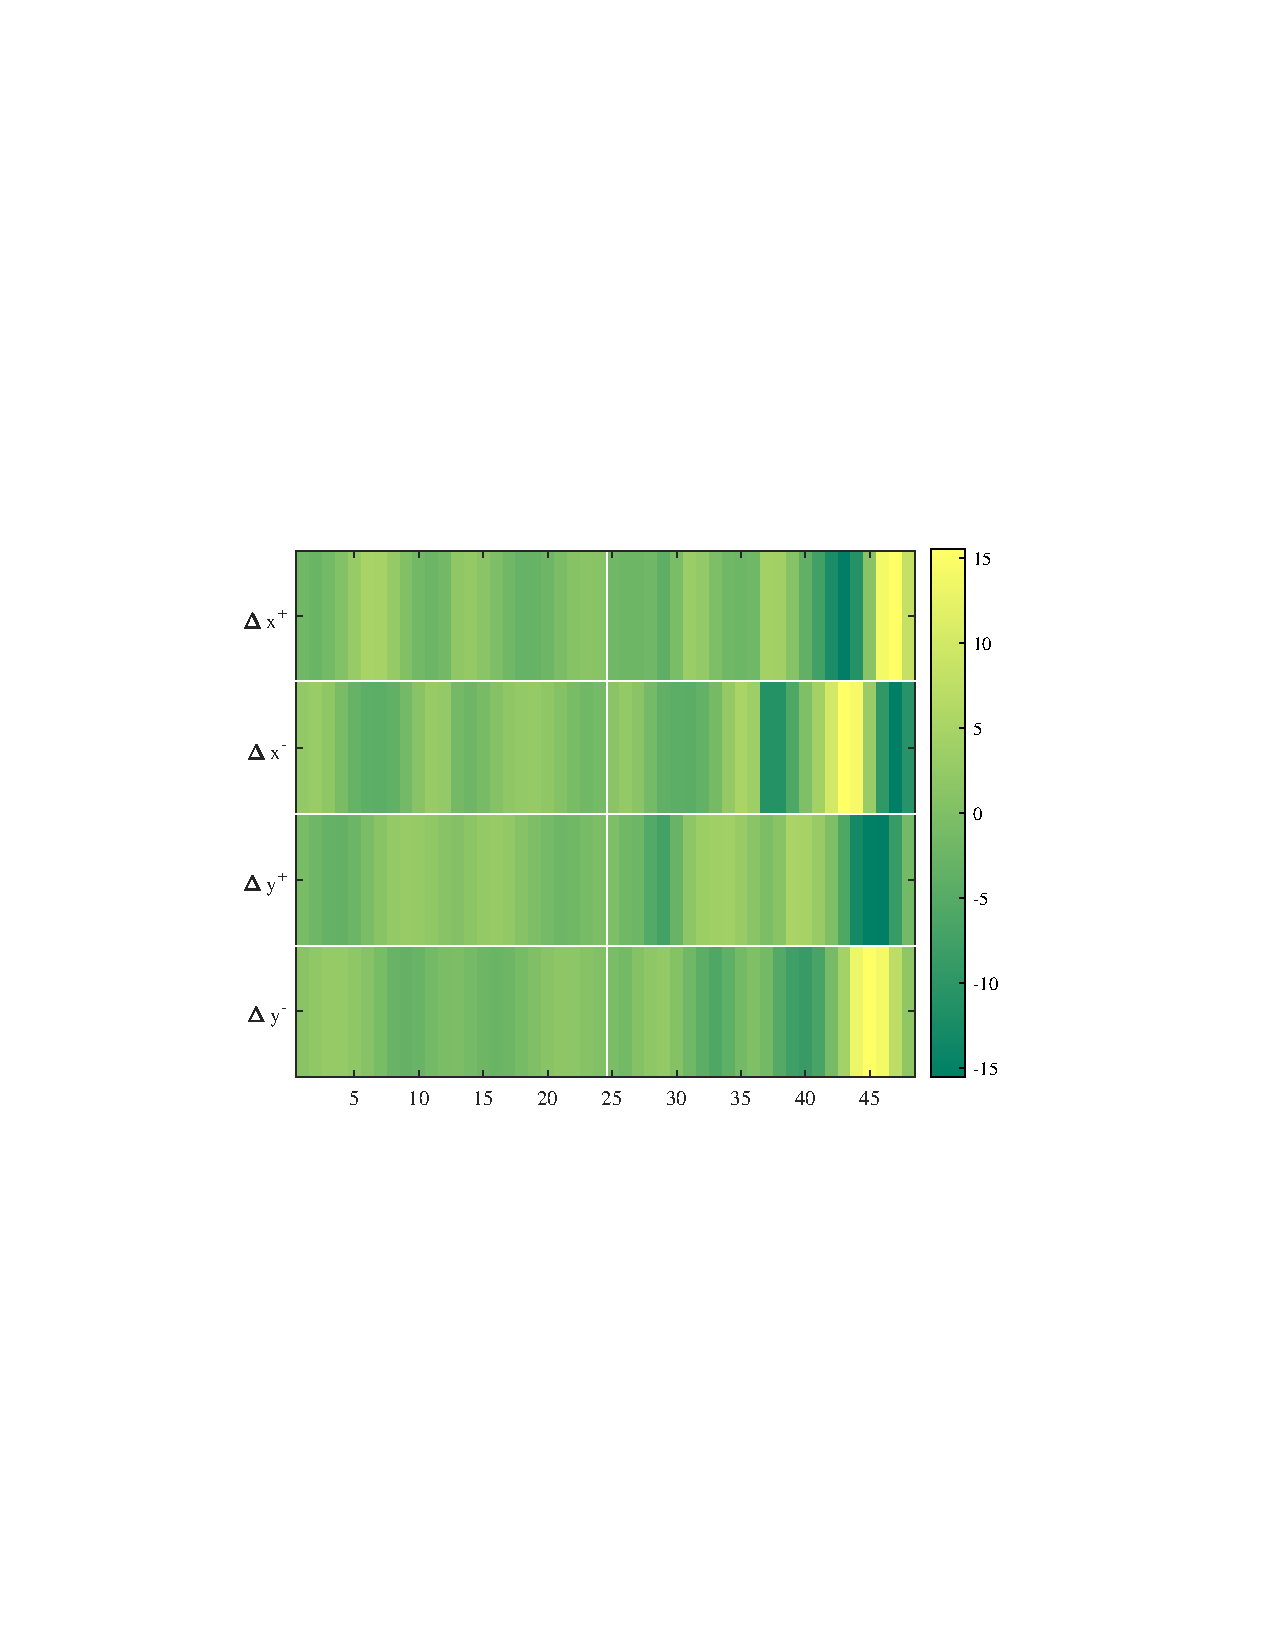
\includegraphics[width=\linewidth]{Figures/Synaptic Weights - BRC.pdf}
        \caption{Synaptic Weights before Reward change in \ac{RCSE} method.}
        \label{fig_3_8}
    \end{minipage}
    \hfill
    \begin{minipage}{0.48\textwidth}
        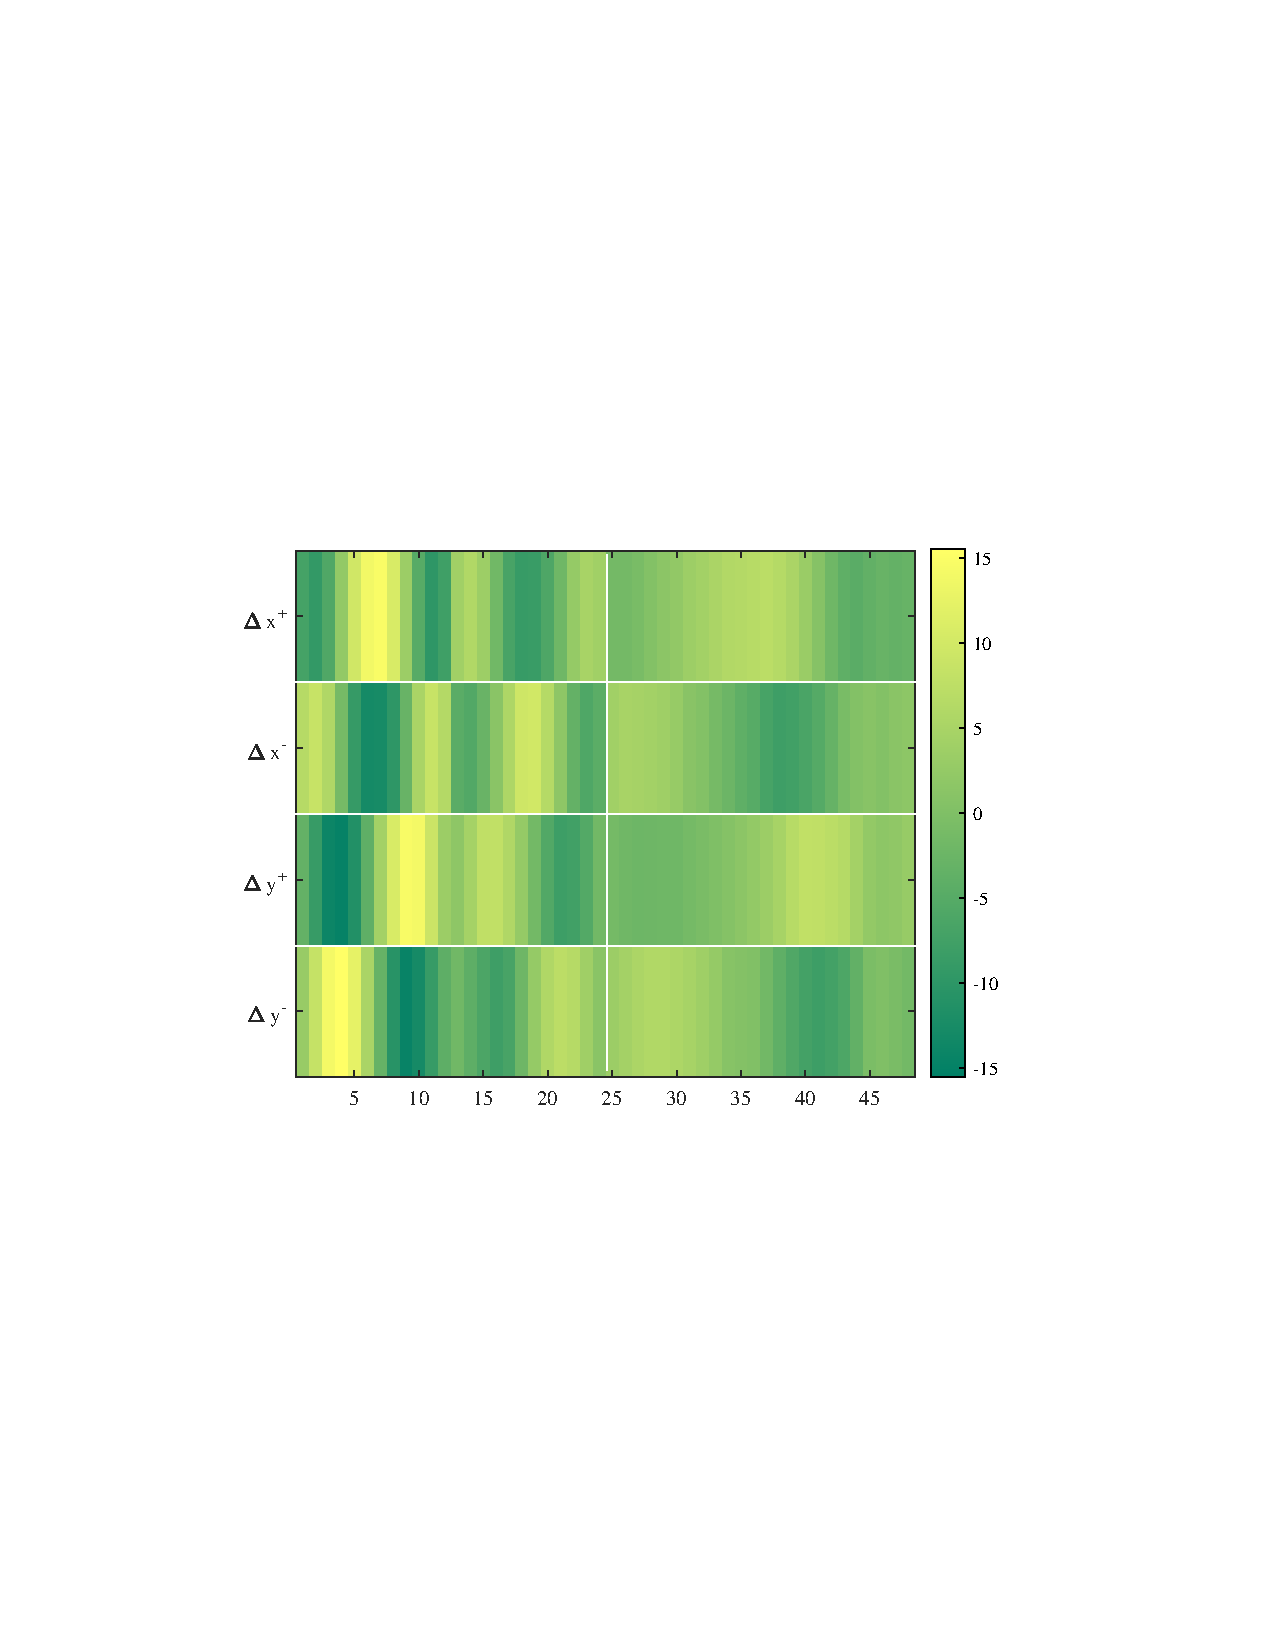
\includegraphics[width=\linewidth]{Figures/Synaptic Weights - ARC.pdf}
        \caption{Synaptic Weights after Reward change in \ac{RCSE} method.}
        \label{fig_3_9}
    \end{minipage}
\end{figure}


\begin{figure}[H]
    \centering
    \begin{minipage}{0.48\textwidth}
        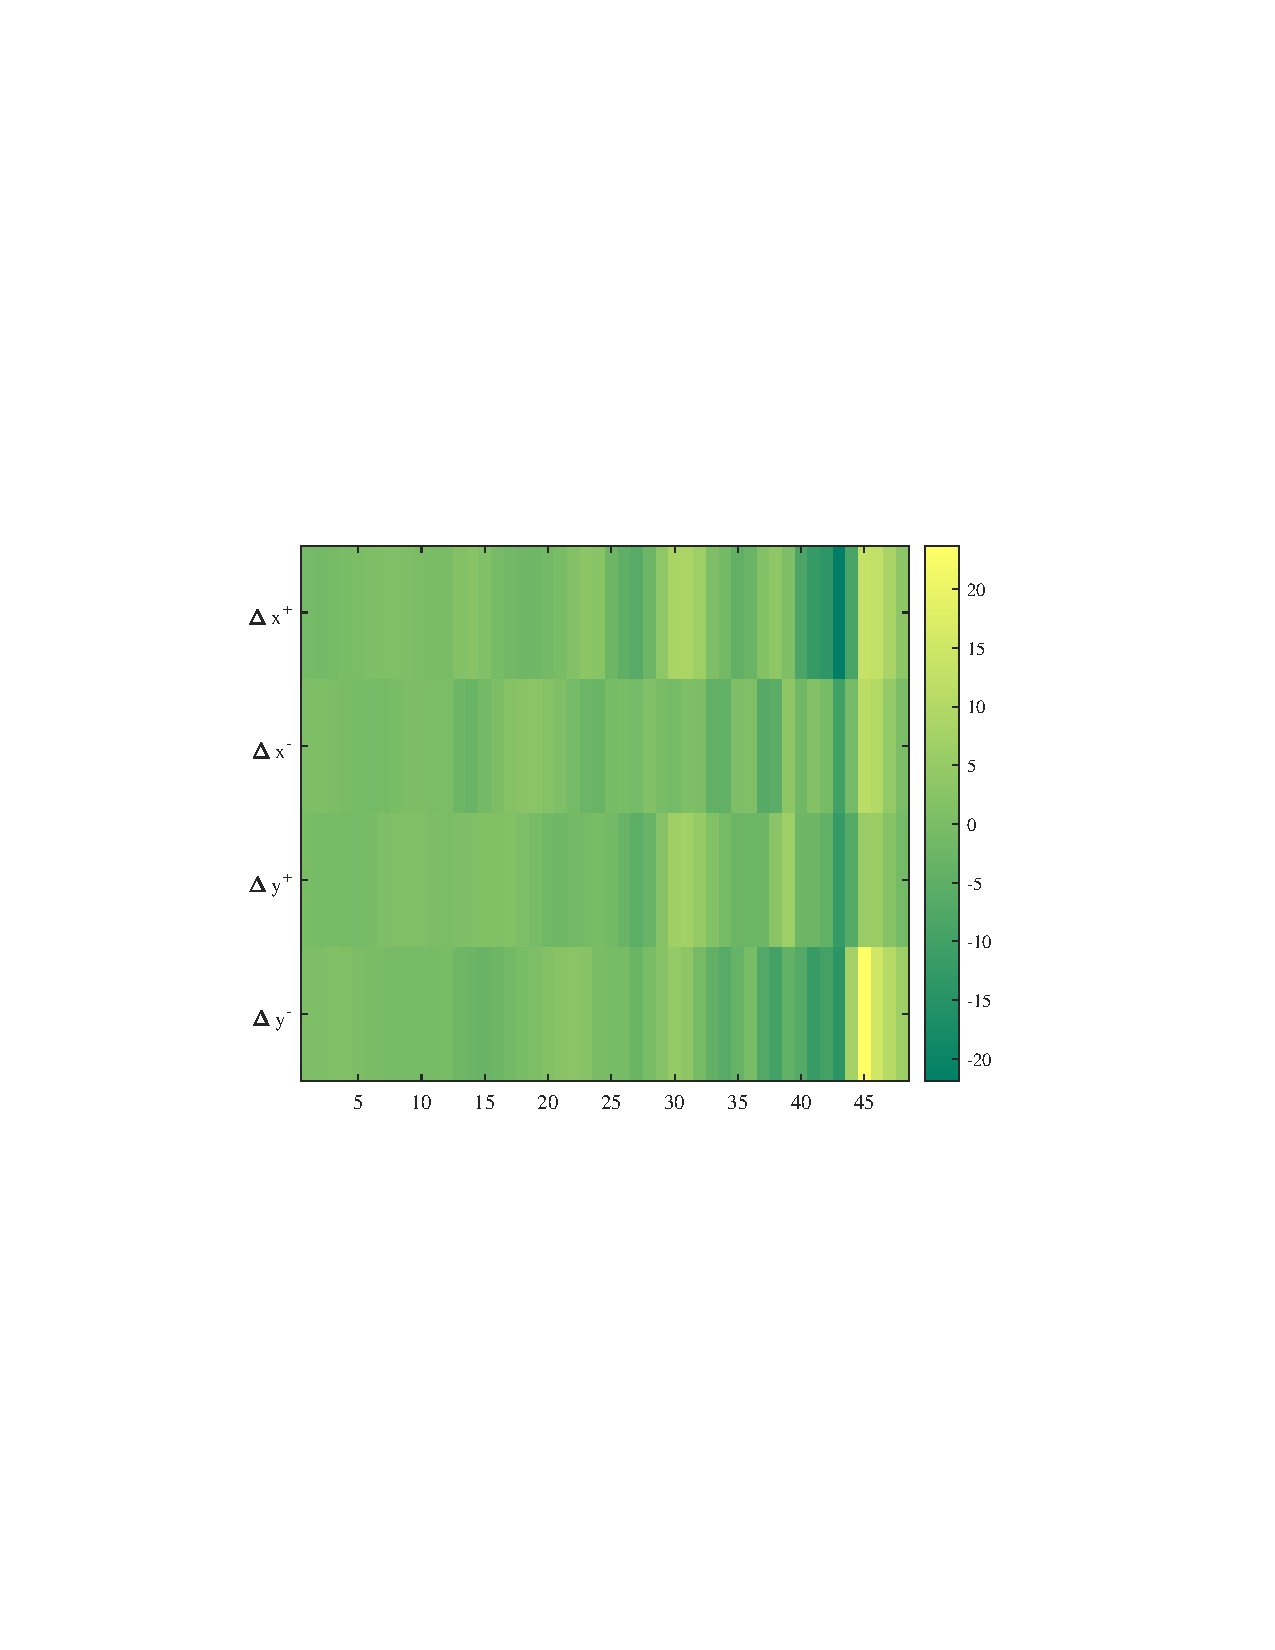
\includegraphics[width=\linewidth]{Figures/MSN - Before Reward Change.pdf}
        \caption{Synaptic Weights before Reward change in Multiplicative Synaptic Normalization method.}
        \label{fig_3_8_1}
    \end{minipage}
    \hfill
    \begin{minipage}{0.48\textwidth}
        \includegraphics[width=\linewidth]{Figures/MSN - After Reward Change.pdf}
        \caption{Synaptic Weights after Reward change in Multiplicative Synaptic Normalization method.}
        \label{fig_3_9_1}
    \end{minipage}
\end{figure}

The visual patterns observed in the synaptic weights matrix in Figure \ref{fig_3_8} and \ref{fig_3_9}, specifically, the gradual increases and decreases in values across weights, directly result from applying Gaussian membership functions for encoding. As illustrated in the heatmap visualization, regions of higher values denote areas closer to the function's center, where the degree of membership peaks. Conversely, areas of lower values reflect points moving away from the center, where the membership degree decreases according to the Gaussian distribution's tails. Figure \ref{fig_3_3_2} further demonstrates this behavior. The differences in synaptic strengths arise from variations in spike rates, reflecting differences in membership degree.

Since the reward coefficients for followers and leaders are different, their maximum allowed synaptic weights are also different. The proposed method given by \eqref{Eq.WS.4} for controlling the unbounded growth of synaptic weights has successfully stabilized the network.

Figures \ref{fig_3_8_1} and \ref{fig_3_9_1} show the performance of the Multiplicative Synaptic Normalization (MSN) method. According to the results, this method cannot control the weight growth because of the coexistence of the excitatory and inhibitory (positive and negative synaptic weights). This method adjusts the weights when the summation of the input synaptic weights to an output neuron exceeds the maximum synaptic weight. In this case, the condition is never satisfied because positive and negative synaptic weights cancel each other, which is why we see synaptic weight values around 30 or -50 that are not within the $I^{minimum}$ and $I^{maximum}$ range. According to Figure \ref{fig_3_9_1}, when the reward changes for the Leader, the MSN cannot adjust the weights because it does not have the reward-modulated decay rate mechanism.

\begin{figure}[H]
    \centering
    \begin{minipage}{0.48\textwidth}
        \includegraphics[width=\linewidth]{Figures/RLST - Weight Increase.pdf}
        \caption{Synaptic weights increase after reward change in \ac{RCSE} method.}
        \label{fig_3_10}
    \end{minipage}
    \hfill
    \begin{minipage}{0.48\textwidth}
        \includegraphics[width=\linewidth]{Figures/RLST - Weight Decrease.pdf}
        \caption{Synaptic weights decrease after reward change in \ac{RCSE} method.}
        \label{fig_3_11}
    \end{minipage}
\end{figure}


Figures \ref{fig_3_10} and \ref{fig_3_11} show the synaptic weights after the reward change (change in environment). In this case, since the reward coefficients are changed, the \(\eta\) and \(\beta\) values in \eqref{Eq.WS.3.1} are changed for the represented sub-layers, and the proposed method has helped the \ac{stdp} algorithm to adjust the weights based on the new situation in the environment.

\subsection{Simulation with Federated Learning and Reward-modulated Competitive Synaptic Equilibrium}

In this section, the proposed aggregation algorithm is tested. In this case, the agents only send their models when the Euclidean distance between the current and previously published model or the latest global model reaches a threshold. In the first phase, the simulation was done in 600 seconds, and the agents learned to follow the leader. The threshold for publishing the agents' and server models (\eqref{Eq.AFL.4} and \eqref{Eq.AFL.5}) was 0.0005 and 0.00051, respectively. The reason for choosing the server's threshold higher than the agents' is that as soon as the first agent sends its model to the server, the Euclidean distance between the current and previously published model by the server reaches 0.0005, and the server distributes the model immediately. Therefore, the serve's threshold is set higher than the agents' threshold, so it waits for the other agents to send their models.

Figure \ref{fig_3-7} shows the distances between agents and the leader before the reward change, indicating that the agents converge to the solution faster than in the scenario where federated learning has not been used, without any error. Figure \ref{fig_3-8} shows the simulation results for the reward change scenario, indicating that the proposed event-triggered \ac{fl} method has improved the learning performance, enabling the swarm to converge to the solution in 6 seconds. In this case, the neural network learned the policies in less time while preserving the performance.

\begin{figure}[H]
    \centering
    \begin{minipage}{0.48\textwidth}
        \includegraphics[width=\linewidth]{Figures/Distances - BRC - DAI.pdf}
        \caption{Distances during the test phase before reward change in the proposed event-triggered \ac{fl} method.}
        \label{fig_3-7}
    \end{minipage}
    \hfill
    \begin{minipage}{0.48\textwidth}
        \includegraphics[width=\linewidth]{Figures/Distances - ARC - DAI.pdf}
        \caption{Distances during the test phase after reward change in the proposed event-triggered \ac{fl} method.}
        \label{fig_3-8}
    \end{minipage}
\end{figure}

The norm of the synaptic weights can represent the changes in the synaptic weights due to the change in the environment during the training process, which can be used to adjust the learning process in SNNs. In the proposed event-triggered \ac{fl} method, agents communicate with the Central Server (leader) during training. According to Figure \ref{fig:3-10}, the aggregation step time is small at the beginning of the training and increases as the \ac{snn} models converge to the final solution. The rate of change of the norm of the synaptic weights (change in Frobenius norm showed in \eqref{Eq.AFL.3}) determines the communication sample time of the aggregation process, which results in small aggregation intervals when the change rate is high and larger intervals when it reduces.

\begin{figure}[H]
    \centering
    \begin{minipage}{0.48\textwidth}
        \includegraphics[width=\linewidth]{Figures/Norm.pdf}
        \caption{Frobenius norm of the Agent 1's weighs during the learning phase. The reward changes for the Leader after 600 s.}
        \label{fig:3-9}
    \end{minipage}
    \hfill
    \begin{minipage}{0.50\textwidth}
        \includegraphics[width=\linewidth]{Figures/Communication Log.pdf}
        \caption{Communication times for agents and the Central Server (Leader). Red and blue dots show the times that agents and the Central Server have sent their model, respectively.}
        \label{fig:3-10}
    \end{minipage}
\end{figure}


Initially, the aggregation frequency is high, but it decreases as the change in synaptic weights approaches zero. This reduction occurs because the learning rate matrix in (\ref{Eq.WS.1}) also approaches zero. The Sigmoid function is specifically designed to output 0 when the maximum synaptic weight exceeds the threshold and to output 1 when it is below the threshold. Also, after the reward changes and the leader becomes an obstacle after 600 seconds, the Euclidean distance between the converged and current models increases and reaches the threshold. As soon as the first agent sends its model to the server, the aggregation process starts again (change in synaptic weights and the Frobenius norm shown in \eqref{Eq.AFL.3}), and the agents adjust the associated synaptic weight.

\begin{table}[h]
    \centering
    \small
    \caption{Comparative Performance Analysis of the Proposed Aggregation Algorithm+\ac{RCSE} and \ac{RCSE}}
    \begingroup
    \renewcommand{\arraystretch}{1.5}
    \begin{tabular}{lcc}
    \hline
                                & \textbf{FL+\ac{RCSE}} & \textbf{\ac{RCSE}} \\
    \hline
    \textbf{Learning (Convergence) Time - Training Phase (s)}                & 261.92               & 554.71\\
    \textbf{Max Distance Convergence Error - Test Phase (\%)} & 0.71             & 1.95\\
    \textbf{Convergence Time for Distance - Test Phase (s)}             & 5.81           & 8.94\\
    \hline
    \end{tabular}
    \endgroup
    \label{tab:Results analysis}
\end{table}

It should be noted that in the test phase, the synaptic weights oscillate around the converged values. When they are lower than the converged value, the learning rate is 1; otherwise, it is 0. The decay rate pulls them away from the converged value, and the reward pulls them back toward it. The oscillation arises from the hard threshold mechanism, defined by the Sigmoid function. Therefore, if the reward changes (due to environmental changes), synaptic weights can adjust quickly because the learning rate returns to 1. 

Table \ref{tab:Results analysis} compares the results and focuses on three critical metrics: learning time, maximum error after convergence, and convergence time. The proposed \ac{fl} algorithm demonstrates significant improvements in terms of efficiency and accuracy, as evidenced by its considerably shorter learning and convergence times and a notable reduction in error after convergence.

\section{Conclusion}

In this chapter, we presented a comprehensive approach addressing the challenges of uncontrolled growth in synaptic weights (shown in Figures \ref{fig_3_8_1} and \ref{fig_3_9_1}) and the limited responsiveness of \ac{stdp} to real-time changes within \ac{snn}s. Our proposed solution integrates the \ac{RCSE} method with a dynamic aggregation interval in \ac{fl} and significantly reduces learning time while improving performance.

The R-CSE method introduces a novel mechanism to manage the unbounded growth of synaptic weights by dynamically adjusting the decay rate through the SoftPlus function. This adjustment is sensitive to the learning stages and rewards changes, ensuring that synaptic weight adjustments remain responsive over time. By addressing the challenge of synaptic weight saturation, the \ac{RCSE} method facilitates a balanced approach to weight adjustment, preventing network saturation and promoting continuous learning adaptability.

We introduce a novel approach that uses \ac{fl} in SNN and employs the Frobenius norm to adjust weighted aggregation in \ac{fl}. Additionally, we include weight decay proportional to the time elapsed since an agent's last model publication. This improves the efficiency and responsiveness of the learning process.

Our proposed method adjusts its aggregation time based on the Euclidean norm. This metric measures the distance between the weight matrices of the agents and the server, determining reduced intervals for model publication. Our results show that the proposed aggregation method significantly accelerates agents' learning while reducing the distance convergence error (Table \ref{tab:Results analysis}).

Moreover, the dynamic aggregation interval effectively reduces communication overhead between the agents and the central server, particularly after model converges and the algorithm switches from the training mode to the operational mode. This reduction is critical when communication bandwidth is limited or costly. This approach is particularly advantageous in 5G networks, where efficient bandwidth use can enhance the overall throughput and reduce latency in real-time applications. Moreover, the adaptive use of communication resources aligns with the scalable and flexible infrastructure of 5G, optimizing network performance even during peak demand periods.